A prt fájlok betöltéséhez és megjelenítéséhez egy egyszerű alkalmazást készült, 
ami egy darab OpenGL ablakból áll. 
Az ablak funkciója alapvetően a részecskék megjelenítése 
és az animáció lejátszása, 
de van rajta egy két panelból álló felhasználói felület is. 
Az egyik panel a {\ttfamily Settings}, 
amin egyrészt lehetőség van futási időben állítani 
az alkalmazás működésével kapcsolatos fontos paramétereken, 
másrészt ezen történik a betöltendő fájlokat tartalmazó mappa megadása, 
valamint a megjelenítés elindítása és szüneteltetése. 
A másik panel a {\ttfamily Light settings}, 
amin a megvilágítással kapcsolatos paramétereken lehet állítani.

\begin{figure}[h]
\centering
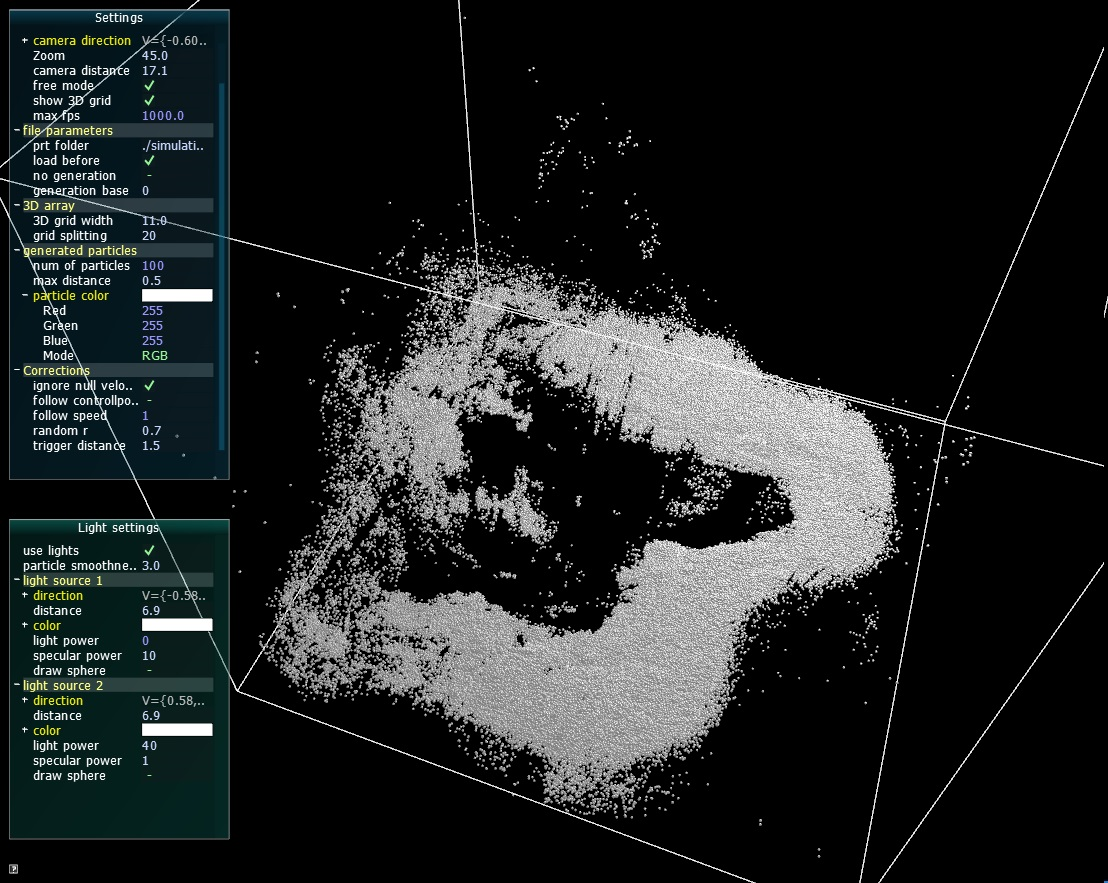
\includegraphics[scale=1.0]{projlab_gui}
\caption{A felhasználói felület}
\label{fig:x projlabGui}
\end{figure}

\section{A prt fájlok betöltése}

Az alkalmazás legfontosabb feladata a prt fájlok betöltése és megjelenítése. 
A felhasználóval való interakció a következőképpen történik:
\begin{itemize}
\item Az alkalmazás a felhasználótól megkapja 
a betöltendő fájlokat tartalmazó könyvtár elérési útját, 
ami a következő kifejezésre illeszkedik:

{\ttfamily "\$\{path\}/\$\{directoryname\}"}

\item Az elérési út végén szereplő {\ttfamily directoryname} alapján 
a program elkezd egymás után fájlneveket generálni
a következő minta szerint:

{\ttfamily "\$\{directoryname\}\_\$\{filenumber\}.prt"}
\end{itemize}
Ahol a {\ttfamily filenumber} egy mindenképp négyjegyű egész szám, 
aminek az elejét a program 0 -kal egészíti ki, 
ha kevés a számjegy. 
A fájlnevek generálása {\ttfamily „0000”} -val kezdődik és addig megy, 
amíg a fájlnév szerinti fájlt be lehet tölteni. 
A \ref{fig:x prtDirectory} ábrán példának 
egy szimulációs fájlokat tartalmazó mappa látható:
\begin{figure}[h]
\centering
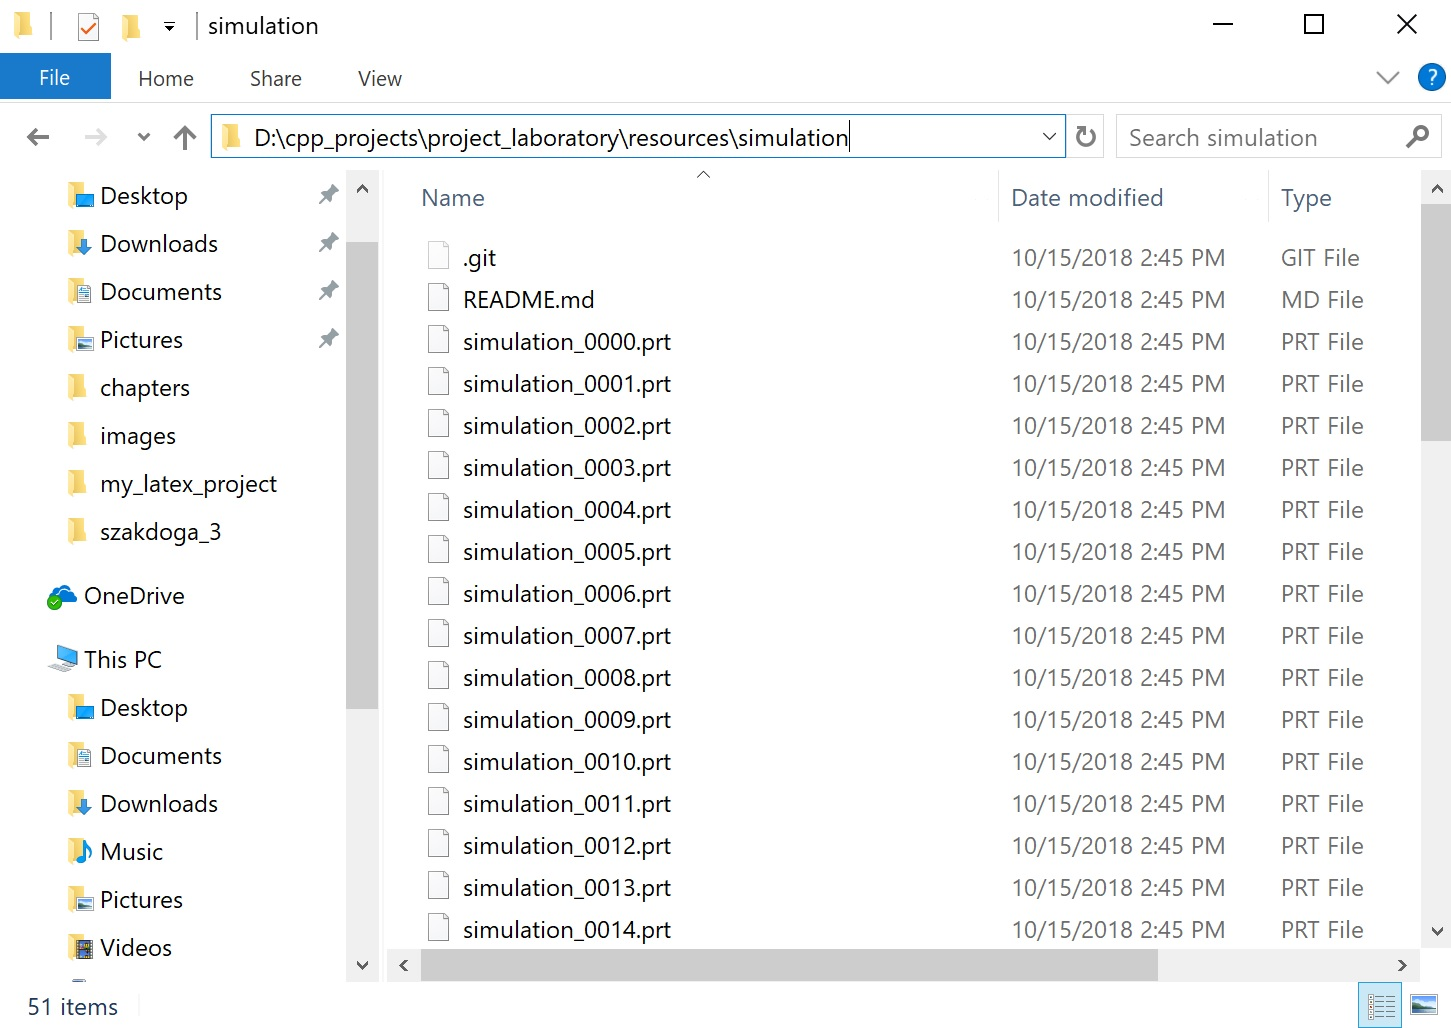
\includegraphics[scale=0.7]{prt_directory}
\caption{A betöltendő mappa}
\label{fig:x prtDirectory}
\end{figure} \newline
Ekkor a betöltéshez a következő elérési utat kell beírni: {\ttfamily c:/simulation}

Az alkalmazásban a fájlok betöltésére két módszer is van. 
Az első, hogy a betöltés gomb megnyomásakor a program végigmegy 
a lehetséges fájlokon és egyszerre betölti 
a memóriába az összeset. 
Ennek előnye, hogy gyors és a háttértárat kevésbé használja. 
A másik lehetőség, 
hogy a program egyszerre csak egy fájl tartalmát rajzolja ki 
és ahogy halad előre, mindig betölt egy újabbat. 
Ez lassabb és folyamatosan terheli a háttértárat, 
ugyanakkor így lehetővé válik nagyon sok nagyon nagy fájl betöltése is, 
amik egyébként együtt nem férnének el a memóriában. 
A gyakorlatban ez szinte soha nem fordul elő, 
így a program alapból az első módszert használja.

\section{A prt fájlok kirajzolása}

A program a prt fájlokat a nevükben szereplő szám szerinti sorrendben tölti be 
és rajzolja ki egymás után. 
A felületen lehetőség nyílik beállítani 
az egy másodpercenként megjelenített fájlok maximális számát,
valamint található egy animáció szüneteltetése opció is.

A részecskék kirajzolására alapvetően két lehetőség van. 
Az egyik,
hogy a program a részecskék helyére Goureaud árnyalt gömböket rajzol, 
amikhez a megvilágítást két pontfényforrás biztosítja. 
Az alkalmazás tartalmaz egy {\ttfamily lights} panelt is, 
amin ilyenkor állítható a fényforrások helye, 
a kibocsájtott fény ereje és színe, valamint a gömbök simasága. 
Az egyes fényforrásokhoz tartozik
egy állítható {\ttfamily specular power} opció, 
amivel a program megszorozza gömbökről visszaverődő spekuláris színt. 
A részecskék kirajzolása megvilágítás nélkül is lehetséges. 
Ekkor a program egyszerűen pixel
méretű pontokat rajzol a részecskék helyére.

\section{A kamera}

A kamerának alapvetően két működési módja van: a kötött és szabad mód. 
Kötött módban a kamera a megjelenítési tér középpontjára néz 
és a középpont körül forgatható. 
Ilyenkor a felhasználói felületen lehetőség van a középpontól való távolság 
és a látószög állítására. 
Kötött módban a kamera mozgása valamennyire irányítható 
a billentyűzet segítségével is. 
A {\ttfamily „w”} és {\ttfamily „s”} gombok segítségével 
a kamerát közelíteni és távolítani lehet a középponttól, 
míg az {\ttfamily „a”} és {\ttfamily „d”} gombok 
a kamerát a középpont körül forgatják. 
A kamera másik működési módja a szabad mód. 
Szabad módban a kamera a belső nézetes játékokhoz hasonlóan mozgatható, 
tehát a kamera orientációját az egérrel lehet irányítani, 
míg a kamera helye a {\ttfamily „w”}, {\ttfamily „a”}, {\ttfamily „s”}, 
és {\ttfamily „d”} gombokkal változtatható. 
Természetesen a látószög beállítására ebben a módban is lehetőség van, 
bár a kamera sajnos akkor is mozog, 
ha a kurzort a felhasználói felület fölött mozgatják.

\section{Részecskék generálása}

A programba belekerült egy részecskegeneráló funkció is. 
Ennek célja, hogy a program a betöltött részecskék 
kezdőpozíciója körül véletlenszerűen generáljon további részecskéket úgy, 
hogy a részecskék kezdeti sűrűségeloszlása nagyjából megmaradjon. 
A program ezután megpróbálja úgy mozgatni a generált részecskéket, 
hogy azok lehetőség szerint a fájlból betöltöttekhez hasonlóan mozogjanak. 
Ezzel elérhető, hogy az animáció 
bár sokkal több részecskét tartalmaz, 
lényegileg nem változik. 
A generálással kapcsolatos fontos paraméterek természetesen 
helyet kaptak a felhasználói felületen is.

\section{Az alkalmazás felhasználói felülete}

A továbbiakban részletezésre kerül, 
milyen opciók és beállítások találhatóak 
a felhasználói felületen és tapasztalat alapján 
milyen értékekkel célszerű használni azokat.

A beállítások egy része belső implementációs részletekre vonatkozik.
Ezek leírása következő fejezetben található. 

\begin{description}[font=\normalfont\itshape\space]
\item [Load file:] A felületen megadott mappából betölti 
a szimulációs fájlokat, 
majd elindítja azok megjelenítését.
\item [Pause:] Megállítja/folytatja az animációt. 
A billentyűzeten az enter gombhoz van kötve.
\item [\textbf{display:}] 
\begin{description}[font=\normalfont\itshape\space]
\item [] 
\item [camera direction:] Kötött módban a kamerát lehet vele forgatni 
a tér középpontja körül. 
Szabad módban nem állítható.
\item [Zoom:] A kamera látószögét állítja.
\item [camera distance:] A kamera távolsága a középponttól.
\item [free mode:] Váltás kötött és szabad kameramód között. 
A billentyűzeten a space gombhoz van kötve.
\item [max fps:] A frame váltások maximális száma másodpercenként. 
A GLFW3 -ban alapvetően 60 a maximális fps érték, 
így annál gyorsabb semmiképp sem lesz.
\end{description}
\item [\textbf{file parameters:}]
\begin{description}[font=\normalfont\itshape\space]
\item [] 
\item [prt folder:] A mappa elérési útja, 
amiben a betöltendő prt fájlok találhatóak.
\item [load before:] Ezzel az opcióval lehet állítani, 
hogy a program a fájlokat előre töltse be és a memóriában tárolja, 
vagy a betöltés külön –külön történjen futási időben.
\item [no generation:] Ha be van jelölve, 
a program nem generál részecskéket a betöltöttek mellé.
\item [generation base:] Az opcióval lehetőség van megadni, 
hogy a részecskék generálása hanyadik frame alapján történjen. 
Ennek alapértelmezett értéke 0, és ott célszerű tartani.
\end{description}
\item [\textbf{3D array:}]
\begin{description}[font=\normalfont\itshape\space]
\item []
\item [3D grid width:] Azon tér szélessége (és magassága), 
amin belül a 3D rácsnak hatása van a generált részecskék mozgására. 
A megadott betöltendő fájlok miatt az alkalmazásban 11 az alapértelmezett érték. 
A teret egyébként egy fehér kocka jelzi, 
így a tér szélessége könnyen változtatható attól függően, 
hogy az animáció mekkora térben játszódik. 
\item [grid splitting:] Meghatározza, 
hogy a 3D rácson belül egy sor/oszlop hány rácspontot tartalmazzon. 
Minél nagyobb a rács szélessége, 
annál nagyobb értéket kell beállítani ugyanazon rácspontsűrűség eléréséhez. 
A betöltendő fájloknál a legjobb eredmény 20 körüli érték mellett keletkezik.
\end{description}
\item [\textbf{generated particles:}]
\begin{description}[font=\normalfont\itshape\space]
\item []
\item [num of particles:] Megadja, 
hogy az egyes vezérrészecskékhez az alkalmazás hány részecskét generáljon.
\item [Max distance:] 
A generált részecske maximális kezdeti távolsága a hozzá tartozó vezérrészecskétől.
\item [particle color:] 
A generált részecskék színe.
\end{description}
\item [\textbf{Corrections:}]
\begin{description}[font=\normalfont\itshape\space]
\item []
\item [ignore null velocity:] 
Bekapcsolt állapotban 
a generált részecskék sebességének meghatározásakor 
csak azok a rácspontok számítanak, 
amikben a beírt sebesség 0 -nál nagyobb. 
A korrekciót célszerű bekapcsolni, 
mivel nélküle a generált részecskék „lemaradhatnak” a vezérrészecskékhez képest.
\item [follow controllpoints:] 
Bekapcsolja a korábban említett korrekciót. 
Ez az opció egyébként önmagában, 
tehát a 3D rács nélkül is biztosíthatja a generált részecskék mozgatását. 
A módszer előnye, 
hogy a generált részecskék a tömegből „megszökő” vezérrészecskéket is követni fogják, 
viszont hátránya, hogy ez a követés túl egyértelműnek tűnhet. 
A 3D rács nélküli használattal további probléma lehet, 
hogy a követés csak késve történik.
\item [Follow speed:] 
Ha a részecske túl messzire kerül 
a hozzá tartozó vezérrészecskétől, 
ezzel a sebességgel kezdi el követni.
\item [random r:] 
A részecske valójában nem közvetlenül a vezérrészecskét követi, 
hanem egy véletlenszerű pontot annak r sugarú környezetében.
\item [trigger distance:] 
A generált részecske ennél a vezérrészecskétől 
való távolságnál kezdi meg a követést.
\end{description}
\item [\textbf{Light settings panel:}]
\begin{description}[font=\normalfont\itshape\space]
\item []
\item [use lights:] Bekapcsolt állapotban 
az alkalmazás a részecskék helyére 
Gouraud árnyalással renderelt gömböket rajzol, 
amikhez a light settings panelen megadott fényforrásokat használja. 
Kikapcsolt állapotban a program egyszínű, 
árnyalás nélküli gömböket fog rajzolni.
\item [particle smoothness:] 
Minél magasabb az érték, 
annál simábbnak fog tűnni a részecskék felülete, 
de túlságosan magas értéket nem érdemes beállítani.
\item [direction:] 
A fényforrást lehet vele forgatni a középpont körül. 
\item [distance:] 
A fényforrás középponttól való távolsága.
\item [color:] 
A fényforrás színe.
\item [light power:] 
A fényforrás ereje.
\item [specular power:] 
A kiszámolt spekuláris színt 
az alkalmazás beszorozza ezzel értékkel és úgy jeleníti meg. 
Azért került az alkalmazásba, 
hogy a részecskék fényesebbnek látszanak 
az alap árnyalási algoritmus kimenete esetén tapasztalhatónál.
\item [draw sphere:] 
Egy gömböt rajzol a fényforrás helyére, 
ami a fényforrás színét veszi fel.
\end{description}
\end{description}

\section{A prt alkalmazáshoz használt eszközök és függvénykönyvtárak}

\vspace{2mm}

\noindent{\itshape\bfseries Git:}

\vspace{2mm}

\noindent A Git egy nyílt forráskódú verziókövető rendszer, 
amit Linus Torvalds kezdett el fejleszteni 2005 -ben 
a linux kernel fejlesztésének támogatásához \cite{wiki:git}. 
Ma már az egyik legelterjedtebb verziókövetőnek számít. 
A prt megjelenítő alkalmazás kódja jelenleg 
egy GitHub repository -n tárolódik és 
a verziókövetés Git -tel történik. 

\vspace{3mm}

\noindent{\itshape\bfseries CMake:}

\vspace{2mm}

\noindent Egy nagyobb, 
több fájlból álló C++ projekt fordítására 
a legkézenfekvőbb megoldás egy shell script írása lenne, 
ami tartalmazza a fordításhoz és linkeléshez szükséges utasításokat. 
Ennek a módszernek több hátránya is lehet:
\begin{enumerate}
\item 
Egy rosszul megírt ad hoc shell script 
minden módosítás után végigfordíthatja az összes fájlt, 
holott csak a módosított 
és az attól függő forráskódfájlok újrafordítására lenne szükség. 
Ez egy több ezer fájlból álló projekt esetén 
jelentősen megnöveli a fordítási időt. 
\item 
Egy nagyobb C++ projekt több külső könyvtártól is függhet, 
amik linkelése egy shell script -ből nehézkes.
\item Gyakran előfordul, 
hogy a kódnak le kell fordulni több különböző környezetben is. 
Erre tipikus példa, 
amikor egy függvénykönyvtár régebbi és újabb verziója között 
interfészbeli különbségek vannak, 
de a programnak le kell fordulnia akkor is, 
ha az adott gépre régebbi verzió van telepítve. 
Ilyen esetekben a shell script -nek el kell tudnia dönteni 
a könyvtár verzióját, 
majd ez alapján definiálnia kell a preprocesszor direktívákat, 
ami jelentősen megnöveli a script komplexitását.
\end{enumerate}
A felsorolt problémákra az egyik lehetséges megoldást 
a unix -szerű környezetekben elterjedt make kínálja. 
Ennek használata egy projekthez adott makefile segítségével történik, 
ami tartalmazza a fordítás szabályait. 
A makefile -ok előnye, hogy nagyon rugalmasak, 
tehát nem csak C++ nyelvhez használhatóak, 
hanem gyakorlatilag bármihez. 
Hátrányuk, hogy egy makefile a shell scriptekhez hasonlóan 
továbbra is feleslegesen hosszú és bonyolult tud lenni.

Windows -os környezetben a megoldást 
az egyes C++ IDE -k beépített szolgáltatásai és 
saját fájlformátumai adják. 
Ilyen a Visual Studio sln, 
vagy a Code Blocks cbp formátuma. Ezek előnye, 
hogy a makefile -okkal ellentétben az sln, 
illetve cbp projektfájlok tartalma 
az adott IDE grafikus felhasználói felületén beállítható, 
tehát nincs szükség semmilyen script -nyelv ismeretére. 
Hátrányuk, hogy így a projekt egy adott operációs rendszer 
adott IDE -jához kötődik, 
tehát például egy sln fájlt tartalmazó projektet csak Windows környezetben, 
kizárólag a Microsoft eszközeivel lehet lefordítani.

A prt megjelenítő alkalmazás fejlesztésekor fontos volt a platformfüggetlenség, 
ugyanakkor jó lett volna, 
ha van lehetőség Visual studio használatára is. 
A megoldást végül a CMake jelentette.
A CMake egy build automatizáló eszköz, 
aminek fejlesztését 1999 -ben kezdte Bill Hoffman, 
aki a VTK könyvtárhoz akkoriban használt 
használt pcmaker -et vette alapul. 
A modern változat, 
amit a prt megjelenítő program is használ, 
2014 -ben jött ki \cite{wiki:cmake}.

\begin{sloppypar}
A CMake használatának legfontosabb előnye, 
hogy egy projekthez adott {\ttfamily CMakeLists.txt} fájl 
alapján képes generálni makefile -t, 
Visual Studio sln projektet, 
vagy akár Code Blocks cbp -t is, 
így biztosítva a projekt operációs rendszer 
és fordítófüggetlenségét. 
A sima makefile -okkal szemben további előny, 
hogy a build script rövidebb és annak írása egyszerűbb.
\end{sloppypar}

Bár a CMake C++ projektekhez az egyik legjobb build eszköz, 
sajnos vannak hiányosságai is például 
az Android projekteknél használt Gradle -höz képest. 
Ezek közül a projekt fejlesztésekor az volt a legzavaróbb, 
hogy nincs lehetőség a függőségek automatikus letöltésére, 
így azokat kézzel kell telepíteni. 
A vtp megjelenítő alkalmazás fejlesztése közben az is kiderült, 
hogy bár a CMake build scriptje egyértelmű 
előrelépés a makefile -okhoz képest, 
a Qt -s qmake -el szemben a szintaktika továbbra is 
feleslegesen bonyolultnak tűnik.

\vspace{3mm}

\noindent{\itshape\bfseries zlib:}

\vspace{2mm}

\noindent A zlib egy tömörítésre és kibontásra használható 
nyílt forráskódú függvénykönyvtár, 
amit Jean-loup Gailly 
és Mark Adler írt 1995 -ben C nyelven \cite{wiki:zlib}. 
Eredetileg a libpng könyvtárhoz készült és a zip fájloknál is 
alkalmazott DEFLATE algoritmust használja.

A függvénykönyvtár hátránya, 
hogy Windows operációs rendszeren alapból nem kerül telepítésre,
így a projekthez külső forráskód függőségként adtam hozzá. 
A projekt szempontjából a zlib -re PartIO függvénykönyvtár fordításához volt szükség. 
A PartIO azért használja a zlib -et, 
mert a prt fájlokban a header rész után a részecskékkel kapcsolatos adatok 
a zlib formátumában vannak tömörítve.

\vspace{3mm}

\noindent{\itshape\bfseries PartIO:}

\vspace{2mm}

\noindent A függvénykönyvtárat részecskefájlok betöltésére írta 
a Walt Disney Animation Studios -nál dolgozó Andrew Selle. 
A könyvtár egy absztrakciós felületet biztosít, 
13 -féle formátumú részecsketároló fájl betöltésére.

A projekt a PartIO -t természetesen a prt fájlok betöltésére használja. 
Sajnos a függvénykönyvtár a fájlbetöltő alkalmazás írásakor még 
elég kezdetleges állapotban volt, 
így bár elvileg a CMake biztosítaná a platformfüggetlenséget, 
gyakorlatilag csak Linux -on lehetett lefordítani.
Windows -on a legnagyobb problémát az jelentette, 
hogy a prt betöltő funkciót teljesen kivették belőle 
egy macro segítségével. 
Ennek oka, hogy Windows -on a prt fájlok kitömörítését végző 
zlib a Linux és MacOS operációs rendszerekkel szemben 
alapesetben nem kerül telepítésre. 
További gondot jelentett egy hiba az egyik fájlban, 
aminek következtében a részecskék 
nem a megfelelő pozíción jelentek meg. 
Mindez azt jelentette, 
hogy a prt megjelenítő projekt részeként 
a PartIO -t is módosítani kellett. 

Végül is a gyors és problémamentes fordítás érdekében 
készítettem egy PartioPRTForWindows függvénykönyvtárat is, 
ami a Partio prt betöltő részét tartalmazza úgy, 
hogy az említett hibákat kijavítottam. 
A projektből a többi fájlformátum támogatását és 
a példákat kivettem, 
viszont a Linux támogatás a név ellenére megmaradt.

\vspace{3mm}

\noindent{\itshape\bfseries OpenGL:}

\vspace{3mm}

Az OpenGL egy API kettő és háromdimenziós vektorgrafikus képek renderelésére. 
Eredetileg a Silicon Graphics kezdte el fejleszteni 1992 -ben. 
Bár természetesen implementálható szoftveresen is, 
a modern OpenGL -t alapvetően azzal a szándékkal tervezték, 
hogy az implementáció jól ki tudja használni a mai a gpu -k képességeit.
 
Az alkalmazás az interneten elérhető jó minőségű segédanyagok, 
valamint az olyan lehetőségek, 
mint a hardveresen gyorsított instancing 
és indexelés miatt a 4.5 -as verziót használja.

\vspace{3mm}

\noindent{\itshape\bfseries GLM:}

\vspace{3mm}

Az modern OpenGL egyik hátránya, 
hogy hiányoznak belőle a rendereléshez 
és egyéb számításokhoz szükséges vektor és mátrixműveletek. 
A GLM fejlesztésekor a cél ezen űr betöltése volt. 
A GLM egy matematikai könyvtár, 
ami tartalmazza a grafikus alkalmazások fejlesztéskor 
felmerülő szinte összes 
lehetséges vektor és mátrixműveletet \cite{glmsite}. 
Egyik fontos előnye, hogy a kód kizárólag header fájlokban található, 
így fordítás nélkül hozzáadható a projekthez.

A GLM előnye a többi hasonló 
függvénykönyvtárral (Pl.: Eigen, a Qt beépített osztályai) szemben, 
hogy az osztályok mind névre, 
mind belső struktúra szempontjából megegyeznek az 
OpenGL Shading Language változótípusaival, 
így a GLM osztályai, mint például a vektor és mátrix,
az OpenGL renderelési csővezetékének módosítások nélkül átadhatóak.

A GLM további előnye például az Eigen -nel, 
vagy a Qt beépített megoldásaival szemben, 
hogy az osztályok az immutable mintát követik. 
Ez azt jelenti, hogy a különböző vektor és mátrixműveletek soha 
nem változtatnak az adott objektum állapotán, 
hanem mindig új objektummal térnek vissza. 
Ez a tulajdonság például a kamera belső változóin 
végzett bonyolultabb műveleteknél jelentősen 
megkönnyítette a programozást.

\vspace{3mm}

\noindent{\itshape\bfseries GLFW:}

\vspace{3mm}

Az OpenGL hátránya, hogy a specifikáció nem tartalmaz függvényeket 
olyan alapvető problémákra, 
mint például az OpenGL ablak létrehozása, 
vagy az egér és billentyűzet eseményeinek kezelése. 
A legegyszerűbb megoldást az adott operációs rendszer 
natív API -jának használata jelenthetné, 
azonban ez Windows esetén bonyolult lenne 
és megakadályozná az alkalmazás platformfüggetlenségét. 
Szerencsére manapság rengeteg olyan egyszerűen 
használható függvénykönyvtár létezik, 
ami képes az OpenGL számára egy platformfüggetlen környezetet biztosítani. 
Ezek közül az alkalmazás a GLFW legújabb, 
3 -as verzióját használja. 
A GLFW egy minimálisra tervezett függvénykönyvtár, 
ami csak a két legalapvetőbb funkcióra képes. 
Ezek az OpenGL ablak létrehozása és 
a perifériákkal kapcsolatos események kezelése.

A GLFW népszerűségét a platformfüggetlenségén kívül 
leginkább sebességének 
és egyszerű használatának köszönheti. 
Sok fejlesztőnek az is számíthat, 
hogy a függvénykönyvtár szabad forráskódú 
és az egyik legszabadabbnak számító zlib licensz védi, 
ami gyakorlatilag semmilyen 
megkötést sem tartalmaz a használatára \cite{glfw}.

\vspace{3mm}

\noindent{\itshape\bfseries AntTweakBar:}

\vspace{3mm}

Az AntTweakBar egy függvénykönyvtár, ami egyszerű, 
gyors és könnyen programozható 
grafikus felhasználói felületet biztosít OpenGL projektekhez. 
Jellemzői a platformfüggetlenség, 
a nyílt forráskód és 
az együttműködés szinte az összes egyszerűbb ablakok létrehozását 
támogató függvénykönyvtárral, 
így például a GLFW -vel is.

Sajnos az eredeti AntTweakBar -t nem tartják karban, 
így a GLFW legújabb, 
3 -as verziójával már nem működik együtt. 
A prt megjelenítő alkalmazás szempontjából 
problémát jelentett az is, 
hogy CMake -el nem build -elhető,
mivel nincs hozzá CMakeLists.txt fájl. 
Emiatt az alkalmazás az eredeti helyett 
egy tschw nevű github user 
módosított AntTweakBar -ját használja \cite{anttweakbar}.

\section{Függőségek kezelése a projektben}

A fejlesztés folyamán egy azonnal 
és minden környezetben probléma nélkül forduló projekt volt a cél. 
Sajnos azonban a CMake például 
a Java projekteknél használt Maven -nel ellentétben 
nem támogatja a függőségek automatikus letöltését. 

A problémát végül úgy sikerült megoldani, 
hogy a projekt csak olyan külső könyvtárakat használ, 
amik forráskódja megtalálható GitHub -on 
és CMake -et használnak build eszközként. 
A külső könyvtárak forráskódjai 
a Git submodule szolgáltatásával a prt megjelenítő 
alkalmazás dependencies mappájába lettek linkelve, 
így ha a {\ttfamily git clone} utasítást {\ttfamily -{}-recursive} 
opcióval hívják, 
a külső könyvtárak forráskódja is letöltődik. 
A módszer működéséhez az is kellett, 
hogy a prt megjelenítő alkalmazás {\ttfamily CMakeLists.txt} fájljában 
legyen egy utasítás a külső könyvtárak fordítására és linkelésére, 
amire szerencsére a CMake lehetőséget biztosít, 
ahogy a külső könyvtárak {\ttfamily CMakeLists.txt} 
fájljában található változók beállítására is. 

Az ötlettel sikerült elérni, 
hogy a program egy egyszerű CMake hívás után azonnal 
leforduljon a függőségek telepítése nélkül, 
bármilyen környezetben.

\section{A prt megjelenítő alkalmazás megvalósítása}

Az alkalmazás architektúrájának tervezésekor megpróbáltam 
szétválasztani a számításokat végző részt 
a user input kezelésétől és 
az OpenGL specifikus kirajzolással kapcsolatos részektől. 
A cél ezzel alapvetően az eredeti, 
asztali környezetben használt Model-view-controller 
minta követése volt. 
Ez nem sikerült teljesen,
mivel a C++ nyelv sajátosságai, 
valamint az AntTweakBar callback függvény kezelése miatt 
a Controller szerepet egy Controller osztály helyett 
a {\ttfamily main.cpp} függvényei kapták meg. 
Ezen kívül az eredeti MVC mintával ellentétben nem 
a Modell rész frissíti a View -t, 
hanem a View kérdezi le a Modell adatait. 
Ennek következtében az újrarajzolást se a Modell változása, 
hanem a controller -nek megfelelő {\ttfamily main.cpp} függvények indukálják.

A Model és View rész különválasztása mögött az volt a motiváció, 
hogy így a jelenlegi OpenGL alapú View mellé 
később a Modell rész megváltoztatása nélkül 
hozzá lehet adni a projekthez egy Vulkan, 
vagy akár DirectX alapút is. 

\begin{figure}[!htb]
\centering
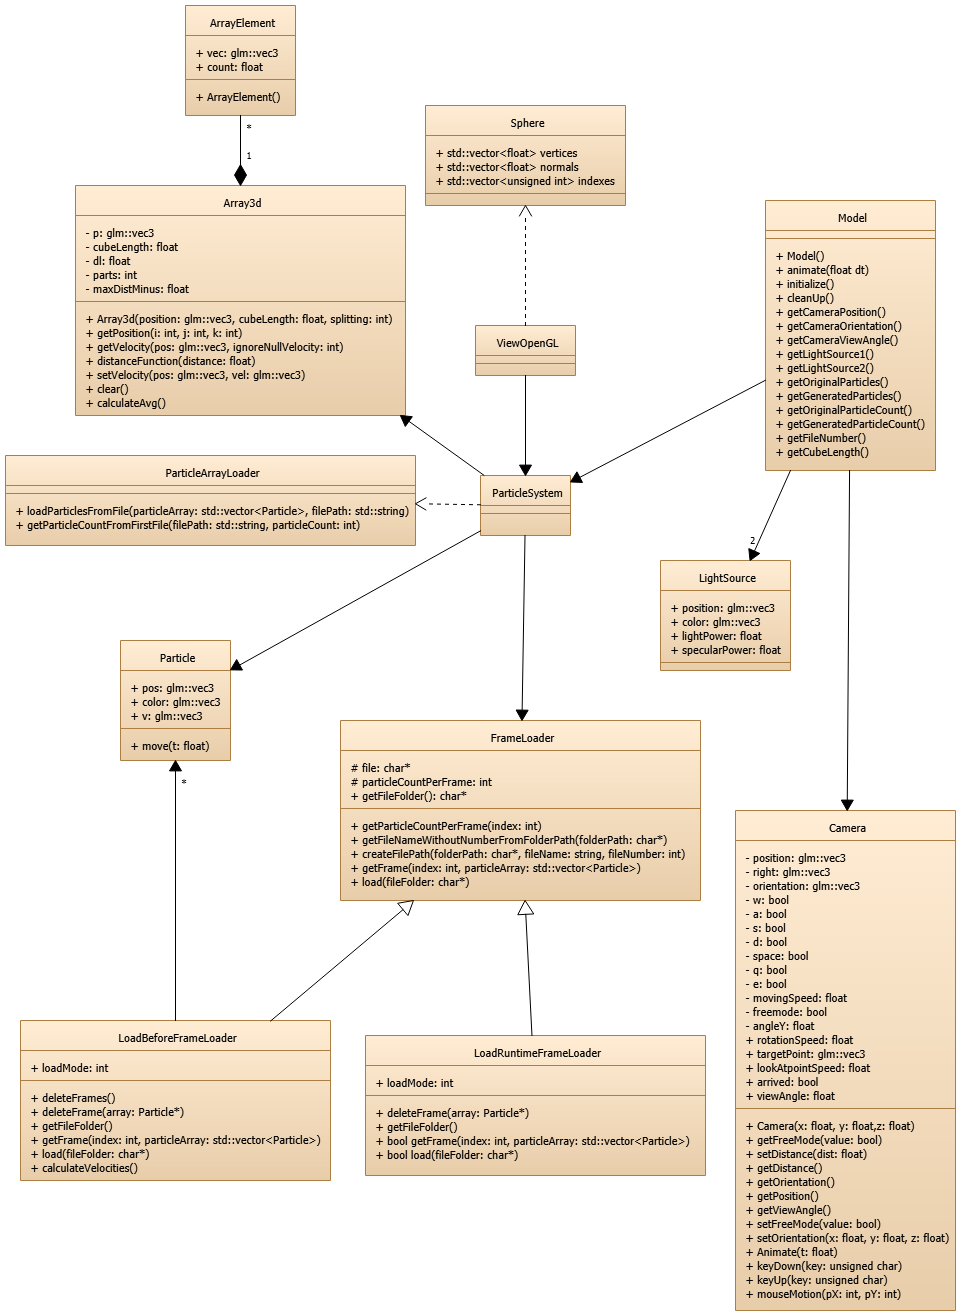
\includegraphics[scale=0.463]{projlab_class}
\caption{Az alkalmazás architektúrája}
\label{fig:x projlabClass}
\end{figure}

\subsection{Az alkalmazás fontosabb osztályai}

\begin{description}[font=\normalfont\itshape\bfseries\space]
\item[Model:] 
Felelőssége a megjelenítési térben található objektumok inicializálása, 
felszabadítása, valamint mozgatása az eltelt idő függvényében. 
A Model osztály kezeli a kamerát és a fényforrásokat is,
mivel ezek helye is függhet az időtől.
\item[LightSource:] 
Egy data class, 
ami a fényforrásokkal kapcsolatos tulajdonságokat tárolja. 
\item[Camera:] 
Feladata, hogy tárolja a kamerával kapcsolatos adatokat, 
valamint itt történik a kamera mozgatása és forgatása is.
Mivel ehhez szükség van az eltelt időre, 
a kamera frissítése és 
tárolása a {\ttfamily Model} osztályban történik.
\item[ParticleSystem:] 
Ebben az osztályban történik a betöltött és generált részecskék 
inicializálása, mozgatása, 
valamint a generált részecskék sebességének kiszámítása.
\item[Particle:] 
Egy data class, 
ami a részecskék pozícióját, 
színét és sebességét tárolja. 
Itt történik a részecske mozgatása is 
a sebesség alapján.
\item[ParticleArrayLoader:] 
Az osztály feladata a részecskék adatainak betöltése 
egy megadott fájlból.
Az osztály jelentősége, 
hogy egy interfész mögé rejti
a PartIO specifikus függvényhívásokat.
\item[FrameLoader:] 
Absztrakt osztály, aminek feladata, 
hogy a megadott mappából betöltse a számozott prt fájlokat. 
Ennek megfelelően itt került megvalósításra
a fájlnevek generálása mappanév alapján. 
Sajnos a megjelenítendő prt fájlokban a sebességek nem voltak megfelelőek, 
így került az osztályba egy sebességszámító funkció is, 
ami a részecskék sebességét az aktuális 
és a következő frame -ben található pozíciók alapján számítja ki.
\item[LoadBeforeFrameLoader:] 
{\ttfamily FrameLoader} leszármazott osztály, 
ami a mappanév megadásakor előre betölti az összes fájlt, 
így a fájlok index szerinti lekérdezése a memóriából történhet.
\item[LoadRuntimeFrameLoader:] 
{\ttfamily FrameLoader} leszármazott osztály, 
ami a mappanév megadásakor pár alapvető értéken kívül (Pl.: részecskék száma) 
nem tölt be semmit. 
A megfelelő fájlok betöltése csak a fájlok index szerinti lekérdezéskor történik.
\item[Array3D:] Ebben az osztályban lett megvalósítva a 3D rács, 
ami alapján a generált részecskék 
fel tudják venni a betöltött részecskék sebességét.
\item[ArrayElement:] 
Egy data class, 
ami egy rácspontnak felel meg. 
Tartalmaz egy sebességvektort és egy súlyösszeget. 
\item[ViewOpenGL:] Az osztály feladata a felhasználói felületet leszámítva 
a megjelenítési tér kirajzolása a Model által szolgáltatott adatok alapján. 
Az osztály felelőssége ezen kívül 
az összes OpenGL specifikus függvény elrejtése a többi rész elől, 
beleértve az OpenGL inicializálását és felszabadítását is.
\item[Sphere:] 
Az osztály feladata, 
hogy egy gömb rendereléséhez biztosítsa az OpenGL számára a vertex, 
index és normal bufferek tartalmát. 
A funkciót a program a részecskék és 
a fényforrások kirajzolásához használja. 
Az osztály használatának előnye a kirajzolandó gömb 
fájlból történő betöltésével szemben, 
hogy így lehetőség van tetszőleges, 
akár futási időben is változtatható háromszögsűrűség elérésére.
\item[main.cpp:] 
Ez nem osztály, 
de végül is ebben a fájlban lettek megvalósítva olyan fontos funkciók, 
mint az OpenGL ablak létrehozása, a fontos osztályok 
és az AntTweakBar inicializálása, 
valamint az eltelt idő nyilvántartása. 
Itt található a GLFW eseményhurokja, 
amiben a Model mozgatása és a ViewOpenGL kirajzoló függvényének meghívása történik. 
A {\ttfamily main.cpp} -ben történik
az alkalmazás objektumainak és függvénykönyvtárainak 
felszabadítása is.
\end{description}

\subsection{A kamera implementálása}

Rendereléskor a kamera aktuális állapotát alapvetően három változó határozza meg. 
Ezek a pozíció és orientáció vektorok, 
amik a kamera helyét és irányát tárolják világ koordinátarendszerben, 
valamint a látószög. 
A fejlesztéskor felmerült a kvaternió alapú kamera is, 
azonban végül nem ez került a programba, 
mivel például a felfele mutató vektor iránya sose változik. 
Ezenkívül a vektor alapú kamera egyszerűbben implementálható 
és a program futása közben kevesebb számítást igényel. 
Az osztályban található egy normalizált jobb vektor is, 
ami mindig merőleges 
a felfele és előre vektorok által kifeszített síkra. 

A kamerába nem került be a V és P mátrixok kiszámítása, 
így a kamera állapotához a {\ttfamily getPosition()}, 
{\ttfamily getOrientation()} és 
{\ttfamily getViewAngle()} függvényekkel lehet hozzáférni. 
Ennek oka, 
hogy a V és P mátrixok kiszámítási módja már függ a használt 
grafikus API -tól (DirectX esetén például máshogy vannak a tengelyek), 
így ez a {\ttfamily ViewOpenGL} osztályba került.

\vspace{3mm}

\noindent{\itshape A kamera mozgatása:}

\vspace{3mm}

A kamera mozgását két darab skalár változó határozza meg. 
Ezek a mozgási és forgási sebesség. 
Kötött módban az {\ttfamily „a”} és {\ttfamily „d”} gombok 
lenyomására a kamera az y tengely körül forog a forgási sebesség szerint,
míg a {\ttfamily „w”} és {\ttfamily „s”} gombok 
hatására a kamera egyszerűen közeledik, 
illetve távolodik az origótól a mozgási sebességnek megfelelően. 
Szabad módban a kamera a {\ttfamily „w”} 
gombra az orientáció vektor, 
míg {\ttfamily „s”} gombra azzal ellentétes irányban mozog. 
Az {\ttfamily „a”} és {\ttfamily „d”} gomb lenyomásakor 
a mozgás a jobb vektorral megegyező, 
illetve azzal ellentétes irányú lesz. 
A programban több gomb lenyomásával elérhető, 
hogy a lenyomott gomboknak megfelelő sebességek összeadódjanak és 
így a sebességvektor az eredő irányba mutasson. 
Ennek megfelelően például a {\ttfamily „w”} és {\ttfamily „s”} gombok 
egyszerre történő lenyomása 0 eredő sebességet eredményez, 
míg a {\ttfamily „d”} és {\ttfamily „w”} gomboknál 
ugyanez egy a jobb vektorral 45 fokot bezáró mozgási irányt fog jelenteni. 
Ha a sebesség irányvektora nem nullvektorra jön ki, 
a sebességvektor hossza minden esetben a mozgási sebesség abszolút értékével 
fog megegyezni.

\vspace{3mm}

\noindent{\textit{Ráfordulás a középpontra 
szabad módból kötött módba történő váltáskor:}}

\vspace{3mm}

Ha az alkalmazásban a felhasználó szabad módból kötött módba vált, 
a kamera a megjelenítési tér közepére fordul. 
A ráfordulás egy forgási animációval történik egy előre beállított sebesség szerint.

\noindent{A középpontra forduláshoz a program a következő algoritmust alkalmazza:
\begin{enumerate}
\item Kiszámolja a kamera pozíciójából a középpontba mutató vektort.
\item Kiszámolja a tengelyt, 
ami körül forgatni kell a kamera irányvektorát, 
hogy az forgatás után pont a középpontba nézzen. 
Ez úgy történik, 
hogy vektoriális szorzással összeszorozza 
a középpontba mutató vektort az irányvektorral.
\item A kamerának átadott eltelt időt beszorozza 
a forgási sebességgel, 
ami a forgatás mértéke lesz radiánban. 
A program ezután kiszámítja az új, elforgatott irányvektort, 
miközben megtartja a régit is.
\item Ellenőrzi, hogy az irányvektor új értéke 
túlfordulna -e a középponton, 
vagy elérné -e azt. 
Ez úgy történik, 
hogy az irányvektor új értékét 
keresztszorozza azzal a vektorral, 
ami a kamera pozíciójából a középpontba mutat. 
Ekkor ha túlfordulás történt, 
a kapott vektor a forgatási tengellyel ellentétes irányba fog mutatni. 
Persze a kicsi értékek miatt a gyakorlatban ez nem lesz teljesen pontos, 
viszont ami biztos, hogy a kapott vektor és 
a forgatási tengely által bezárt szög túlfordulás esetén 
90 foknál nagyobb lesz, 
míg egyébként 90 foknál kisebb (vagy egyenlő). 
A két vektor közbezárt szögét az algoritmus skaláris szorzással ellenőrzi.
\end{enumerate}
}

\subsection{A részecskék kirajzolása}

A részecskék megjelenítése gömbök kirajzolásával történik, 
amihez a program természetesen kihasználja 
a modern OpenGL indexelés és instancing funkcióit.

\vspace{3mm}

\noindent{\textit{Indexelés:}}

\vspace{3mm}

A lehetőség biztosítja, 
hogy ha egy adott pont több, 
egymással határos háromszögben is szerepel, 
akkor is elég legyen egyszer betölteni a bufferbe, 
így a buffer mérete kisebb, 
míg betöltési ideje rövidebb lehet. 
A megoldás hátránya, 
hogy ilyenkor a háromszögpontok megadása indexek segítségével történik, 
amikhez szükség van egy indexbufferre is. 
Mivel viszont egy pont tárolásához kilenc lebegőpontos változóra van 
szükség, 
ezek együtt jóval több helyet foglalnak, 
mint egy darab 32 bites egész szám. 
Az indexelés emiatt általában hatékonyabb adattárolást 
és gyorsabb programot eredményez.

\vspace{3mm}

\noindent{\textit{Instancing:}}

\vspace{3mm}

Az OpenGL instancing szolgáltatása lehetővé teszi, 
hogy egy modell pontjait elég legyen csak egyszer, 
a program inicializálásakor betölteni és a futás folyamán 
rendereléskor már csak a modell pozícióját kelljen megadni.

A program a kirajzolás folyamán egyszerre használ indexelést és instancing -et. 
A részecskék kirajzolása úgy történik, 
hogy először inicializáláskor a program betölti 
az OpenGL bufferekbe a megjelenítéshez használt gömb háromszögpontjainak 
a gömb középpontjához viszonyított pozícióit, 
valamint a háromszögpontok normál vektorait. 
Ezután még inicializáláskor feltölti 
a gömbhöz használt index buffert is. 
A program ezután rendereléskor már csak 
a részecskék színeit és pozícióit adja meg az OpenGL -nek.

\subsection{A megvilágítás implementálása}

A program két pontfényforrást használ, 
amiknek a kezelőfelületen beállítható a pozíciója, 
színe és intenzítása. 
A shader -ekben a megvilágítás számítása Gouraud árnyalással történik. 
Ennek oka, 
hogy egyrészt rengeteg részecskét kell megjeleníteni, 
így a fragment shader -ben történő 
számítás lassíthatta volna a programot, 
másrészt mivel a gömbök kis méretűek, 
a különbség például egy Phong árnyaláshoz képest 
nem lenne észrevehető. 

A felületen lehetőség van 
a spekuláris megvilágítással kapcsolatban további 
két paraméter beállítására is. 
Az egyik a {\ttfamily „specular power”}, 
amivel a spekuláris színt lehet felerősíteni, 
a másik a {\ttfamily „particle smoothness”}, 
amivel a gömbfelület simasága állítható.

\subsection{A fájlbetöltés implementálása}

Az aktuális frame -ben található részecskék a programban a 
{\ttfamily FrameLoader} osztálytól kérdezhetőek le. 
A {\ttfamily FrameLoader} -nek alapvetően három fontos függvénye van. 
Az első a {\ttfamily load} metódus, 
ami a {\ttfamily FrameLoader} inicializálását végzi
a paraméterként átvett mappa elérési út alapján.
A második függvény a {\ttfamily getFrame}, 
ami ha a {\ttfamily FrameLoader} már inicializálva van, 
az inicializáláskor megadott mappában található, 
a paraméterként átadott változónak megfelelő frame
tartalmát visszaadja egy {\ttfamily Particle} tömb formájában. 
A {\ttfamily FrameLoader} harmadik fontos függvénye 
a {\ttfamily getParticlesCountPerFrame}, 
ami visszaadja a mappában található első prt fájl részecskeszámát. 
A függvény azért kapott ilyen nevet, mert a program feltételezi, 
hogy ez a részecskeszám a későbbi {\ttfamily Frame} -ekben sem változik.

A {\ttfamily FrameLoader} tervezésekor az volt a cél, 
hogy legyen egy egységes interfész, 
ami a két különböző betöltési módot 
elrejti a {\ttfamily ParticleSystem} elől 
két leszármazott osztályba, 
amik a {\ttfamily LoadBeforeFrameLoader} és a 
{\ttfamily LoadRuntimeFrameLoader} nevet kapták. 
A {\ttfamily LoadBeforeFrameLoader} {\ttfamily load} 
függvénye az átadott elérési út alapján legenerálja a fájlneveket, 
majd egyszerre betölti az összes fájl összes részecskéjét.
Minden prt fájlhoz egy saját részecsketömb tartozik, 
amikből a getFrame -nek ezután csak elég visszaadnia az indexnek megfelelőt.
A {\ttfamily LoadRuntimeFrameLoader} {\ttfamily load} 
függvénye ezzel szemben csak eltárolja a mappa nevét. 
A fájlnév legenerálása és a részecskék betöltése a {\ttfamily getFrame} 
metódusban történik.

\section{Részecskegenerálás a prt fájlokhoz}

A generálás az eredeti, 
fájlokból betöltött részecskék (továbbiakban vezérrészecskék) 
kezdeti pozíciója alapján történik. 
A program minden vezérrészecskéhez a felhasználói felületen 
megadható számú részecskét generál, 
amiket a vezérrészecskék körül helyez el. 
Az elhelyezés három véletlenszerű szám alapján történik, 
amik a távolságot, 
valamint a vízszintes és függőleges szöget határozzák meg. 
A program először vesz egy x irányú egységvektort, 
amit megszoroz a távolsággal. 
Ezután a vektort elforgatja az y tengely körül a vízszintes szöggel, 
majd veszi az elforgatott vektor keresztszorzatát 
az y irányú egységvektorral és 
e körül forgat a függőleges szöggel. 
Az így kapott vektort a program hozzáadja a vezérrészecske pozíciójához, 
ami a generált részecske új pozíciója lesz.

\subsection{A generált részecskék mozgatásának megvalósítása}

A generált részecskék mozgatása egy szabályos 3D rács segítségével történik, 
amit az {\ttfamily Array3D} osztály valósít meg. 
A 3D rács működése röviden következőképpen írható le:
\begin{enumerate}
\item A program végigmegy a vezérrészecskéken 
és betölti sebességüket a környező rácspontokba.
\item A program minden rácspontra kiszámít 
egy átlagos sebességértéket.
\item A generált részecskék új sebessége 
a legközelebbi rácspontokba beírt sebességek 
távolsággal súlyozott átlaga lesz.
\end{enumerate}

\noindent{Az előző három lépés 
részletes leírása:}

\setlist[description]{font=\normalfont\itshape\space}
\begin{description}
\setlength{\parindent}{2ex}
\item [A vezérrészecskék sebességének betöltése a rácspontokba:] \hfill \\
Ez úgy történik, 
hogy a program először megkeresi, 
hogy a részecske pozíciója alapján mely rácspontokba 
kell a sebességét betölteni. 
Ez a legközelebbi és az azt közvetlenül körbevevő rácspontokat jeleni. \\
A rácspontokban két változó található. 
Az egyik a betöltött sebességek összege, 
amik súlyozva vannak az adott részecske rácsponttól való távolságával. 
A másik a súlyok összege. 
A program minden vezérrészecske esetén végigmegy a környező rácspontokon, 
és hozzáadja a megfelelő értékeket a két változóhoz. 
\item [A rácspontra jellemző átlagos sebességérték kiszámítása:] \hfill \\ 
Ez nagyon egyszerű, 
mivel elég minden rácspontnál elosztani a sebességösszeget a súlyösszeggel. 
Ezzel a módszerrel a rácspontoknál ha sok a vezérrészecske, 
egy olyan átlagos sebességérték fog kijönni, 
ami nagyságrendileg megegyezik a környező vezérrészecskék sebességével. 
Ugyanakkor ha csak egy darab vezérrészecske van, 
a rácspontba annak a sebessége fog bekerülni akkor is, 
ha egyébként súlynak a távolság miatt nagyon kicsi érték jött ki.
\item [A generált részecskék sebességének kiszámítása:] \hfill \\ 
A sebességek beírásához hasonlóan a program 
a kiolvasáskor is a részecskéhez legközelebb lévő 
és az azt közvetlenül körbevevő rácspontokat veszi figyelembe. 
A generált részecskék sebessége egyszerűen 
a rácspontokba írt sebességek átlaga lesz, 
amik súlyozva vannak a távolsággal, 
hogy a közelebbi rácspontok jobban számítsanak. 
\end{description}

\subsection{Korrekciós lehetőségek az alkalmazás felületén}

\setlist[description]{font=\normalfont\itshape\space}
\begin{description}
\setlength{\parindent}{2ex}
\item [A 0 sebességértékek figyelmen kívül hagyása:] \hfill \\
A fenti módszerrel az a probléma, 
hogy sok rácspontban a vezérrészecskék 
sebességeinek beírása után is 0 marad az érték, 
így előfordulhat, 
hogy a generált részecskék a kívántnál a környező nullák miatt 
jóval kisebb sebességértéket vesznek fel, 
így lemaradhatnak a vezérrészecskéktől, 
vagy akár meg is állhatnak. 
A problémára egy lehetséges megoldás, 
hogy a program figyelmen kívül hagyja a környező 0 értékű rácspontokat, 
és csak a többiből számolja az átlagot.
\item [A vezérrészecskék követése:] \hfill \\
Ha be van kapcsolva, 
a részecskék ha túl messzire kerülnek 
a hozzájuk tartozó vezérrészecskétől, 
a sebességükhöz hozzáadódik egy nagyjából 
a vezérrészecske irányába mutató vektor.
A vektor kiszámítása úgy történik,
hogy a program a részecskegeneráláshoz hasonló módszerrel 
választ egy véletlenszerű pontot a vezérrészecske körüli gömbön belül 
és a vektor ezen pont irányába fog mutatni.

A felhasználói felületen egyébként 
beállíthatóak az algoritmus paraméterei, 
amik a generált és vezérrészecske közötti maximálisan elfogadható távolság, 
a vezérrészecske körüli gömb sugara, 
valamint a gömbön belüli pont követésének a sebessége.
\end{description}

\section{Tesztelés}

Az alkalmazást leteszteltem részecskegenerálás nélkül,
valamint kontrollpontonként 3, 20 és 100 generált részecskével.
Mind a négy tesztesetnél ugyanazokat a beállításokat használtam.
A generált részecskék maximális kezdeti távolságát 0.3 -ra, 
a rács felosztását 30 -ra, 
a generált részecskék színét pedig fehérre állítottam.
Bár a rácspontok magas sűrűsége biztosította 
a vezérrészecskék viszonylag pontos követését, 
egyes részecskék az animáció folyamán hátramaradtak,
így engedélyeztem a {\ttfamily follow controlpoints} opciót is.

A tesztgépen az első 2 teszt stabilan hozta a 60 fps -t.
A részecskeszám 20 -ra emelésekor az átlagos fps szám 23 -ra csökkent.
A tesztgép a kontrollpontonként 100 részecskét már nem bírta. 
Itt átlagosan 5 fps -t sikerült elérni.

A tesztelés közben az alkalmazásról képeket is készítettem,
amik a megjelenítendő prt fájlok közül az 1., a 11., a 14. 
és a 30. tartalmát mutatják.

\begin{figure}[!htb]
    \centering
    \begin{subfigure}[!htb]{0.32\textwidth}
        \centering
        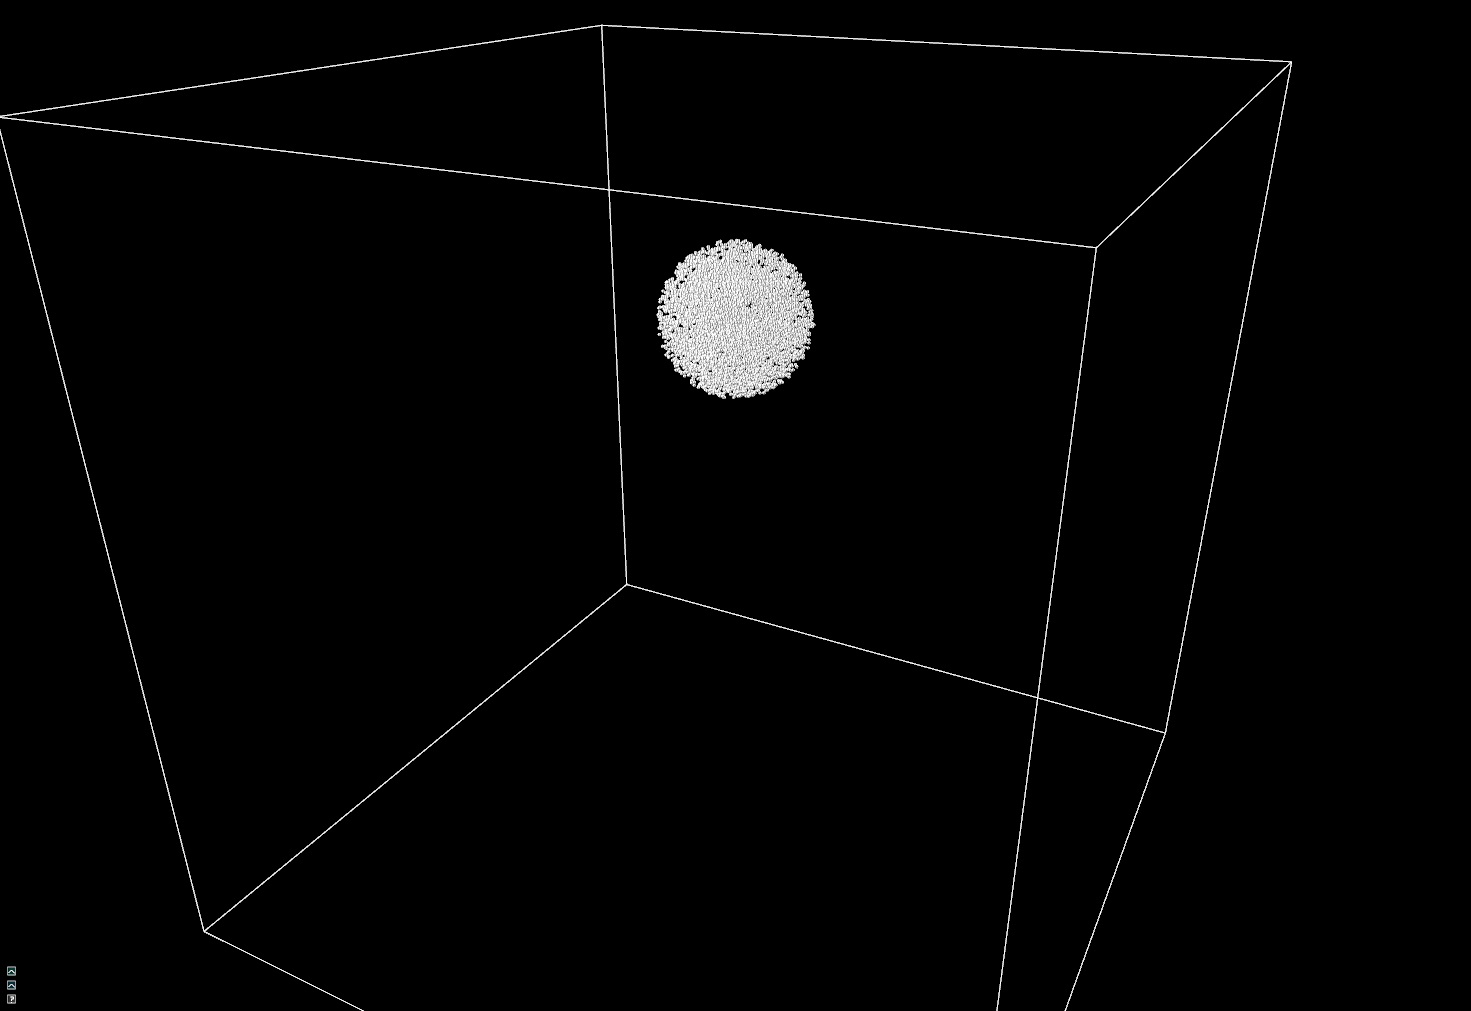
\includegraphics[width=\textwidth]{prt_jpg/1_0}
        \caption{0 részecske}
    \end{subfigure}
    \hfill
    \begin{subfigure}[!htb]{0.32\textwidth}
        \centering
        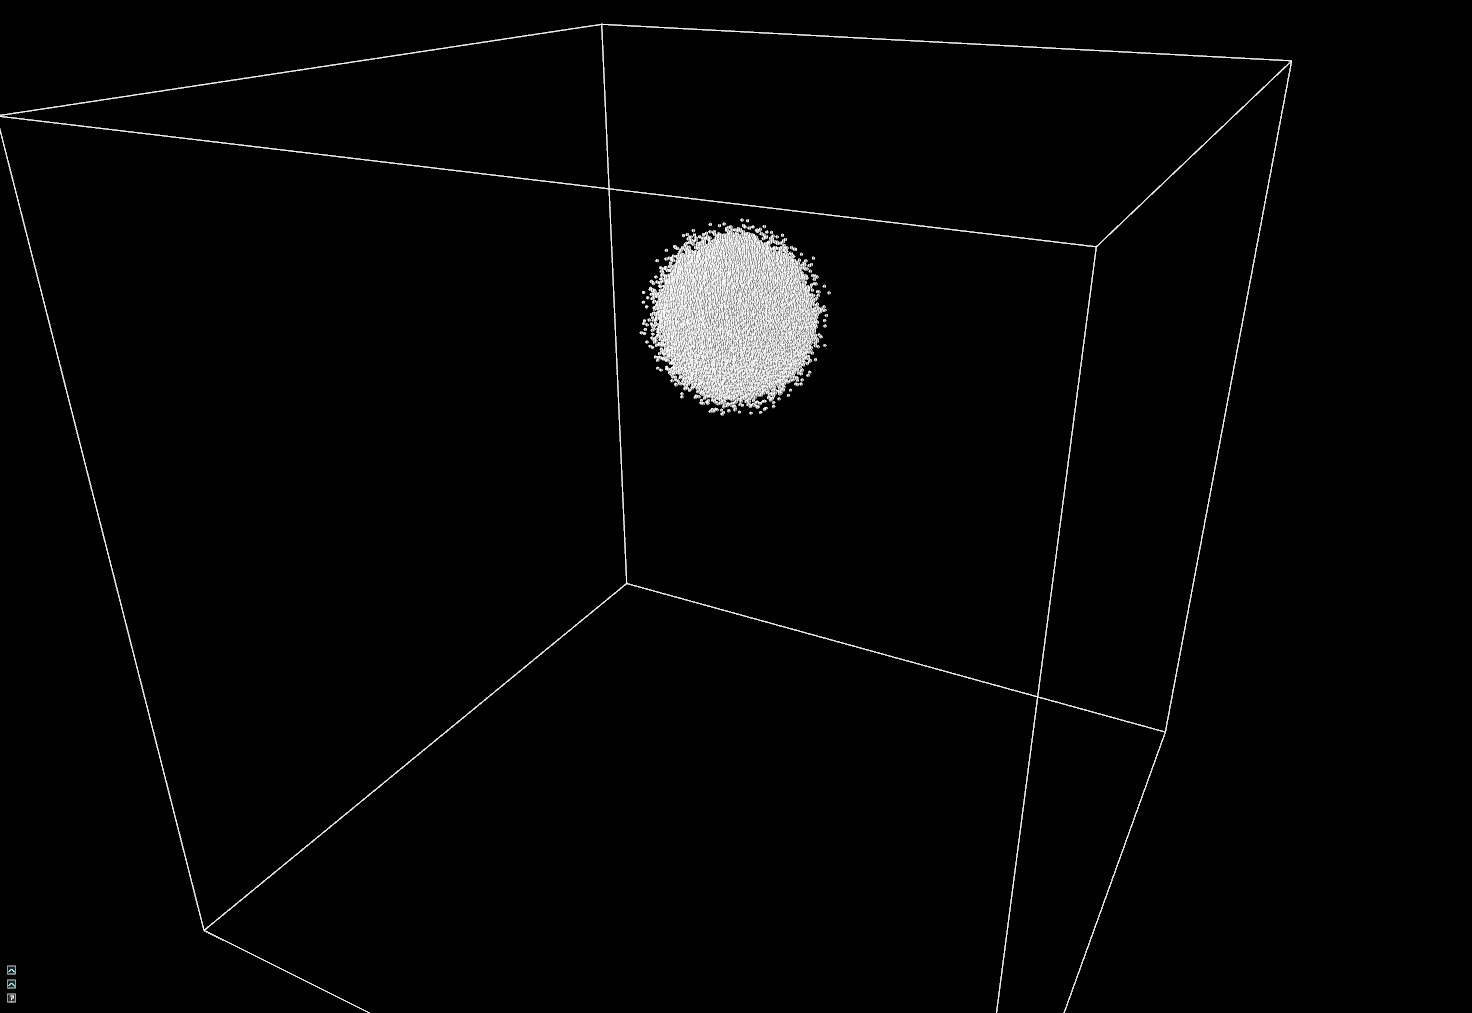
\includegraphics[width=\textwidth]{prt_jpg/1_3}
        \caption{3 részecske}
    \end{subfigure}
    \hfill
    \begin{subfigure}[!htb]{0.32\textwidth}
        \centering
        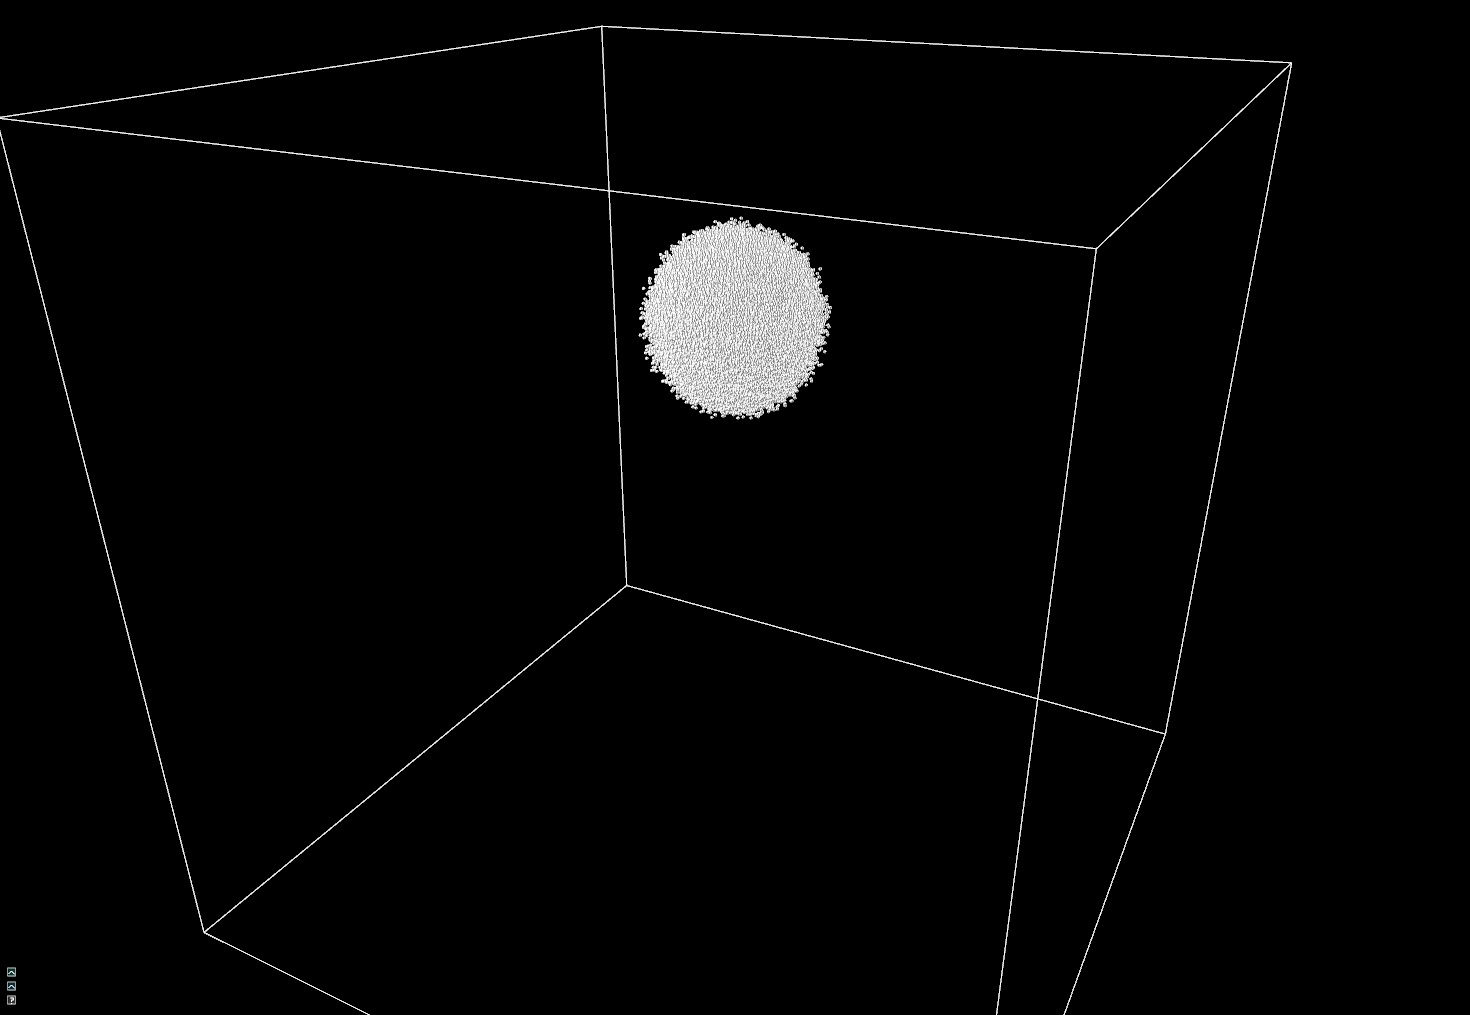
\includegraphics[width=\textwidth]{prt_jpg/1_20}
        \caption{20 részecske}
    \end{subfigure}
    \caption{Az első frame}
    \label{fig:x firstframe}
\end{figure}

\clearpage
{\noindent\itshape A 11. frame:}
\begin{figure}[!htb]
    \centering
    \begin{subfigure}[!htb]{0.32\textwidth}
        \centering
        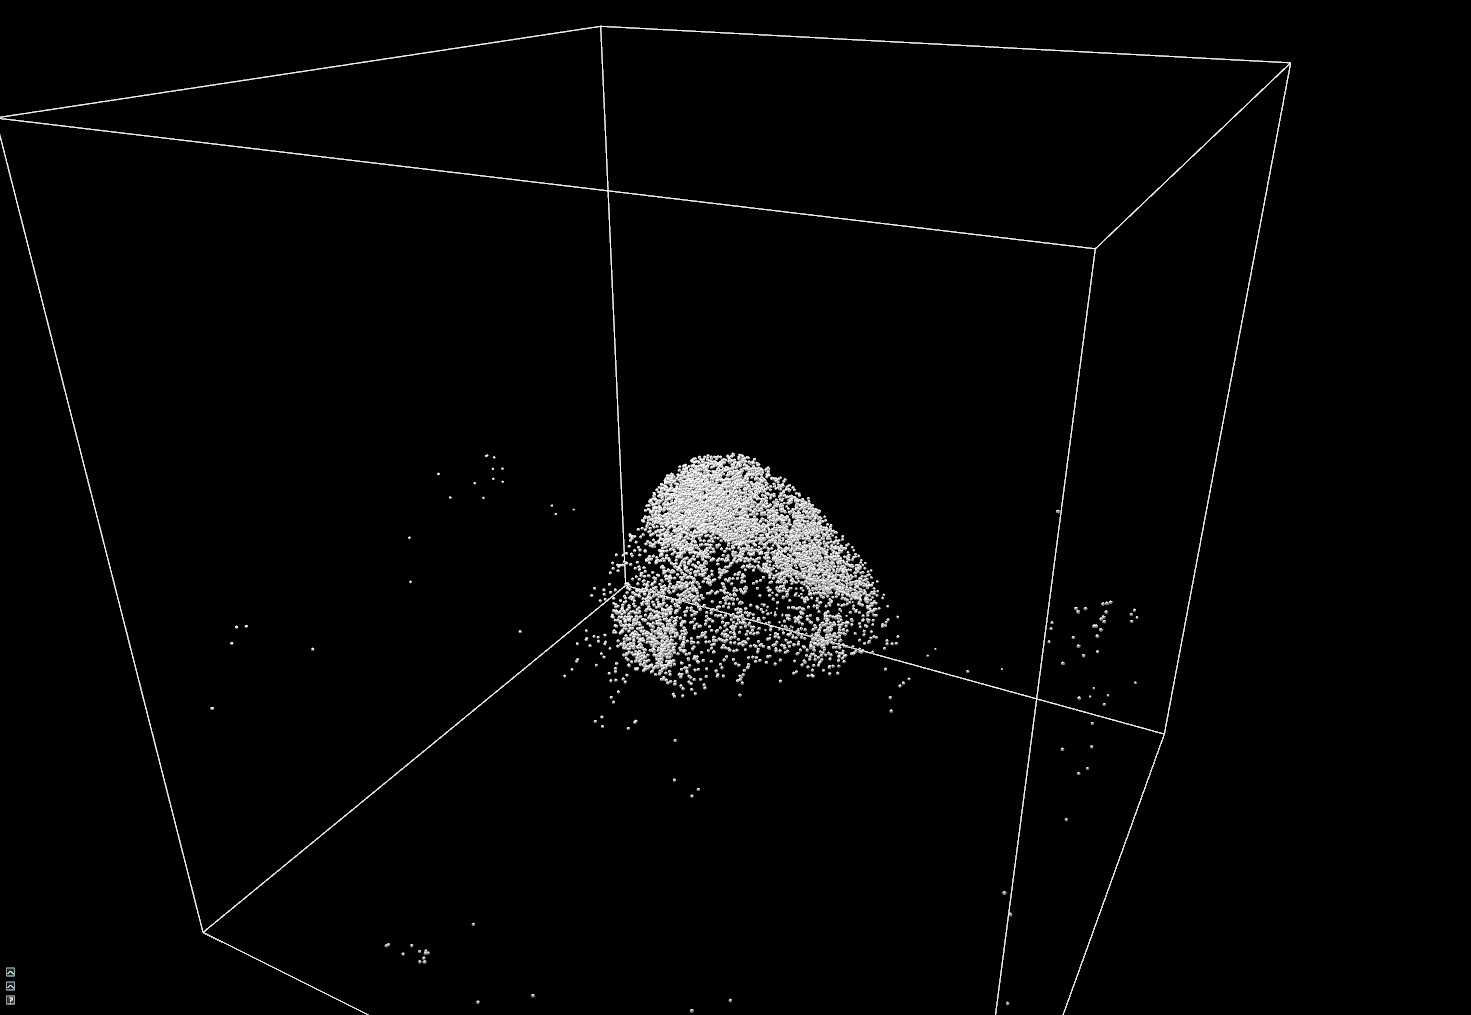
\includegraphics[width=\textwidth]{prt_jpg/11_0}
        \caption{0 részecske}
    \end{subfigure}
    \hfill
    \begin{subfigure}[!htb]{0.32\textwidth}
        \centering
        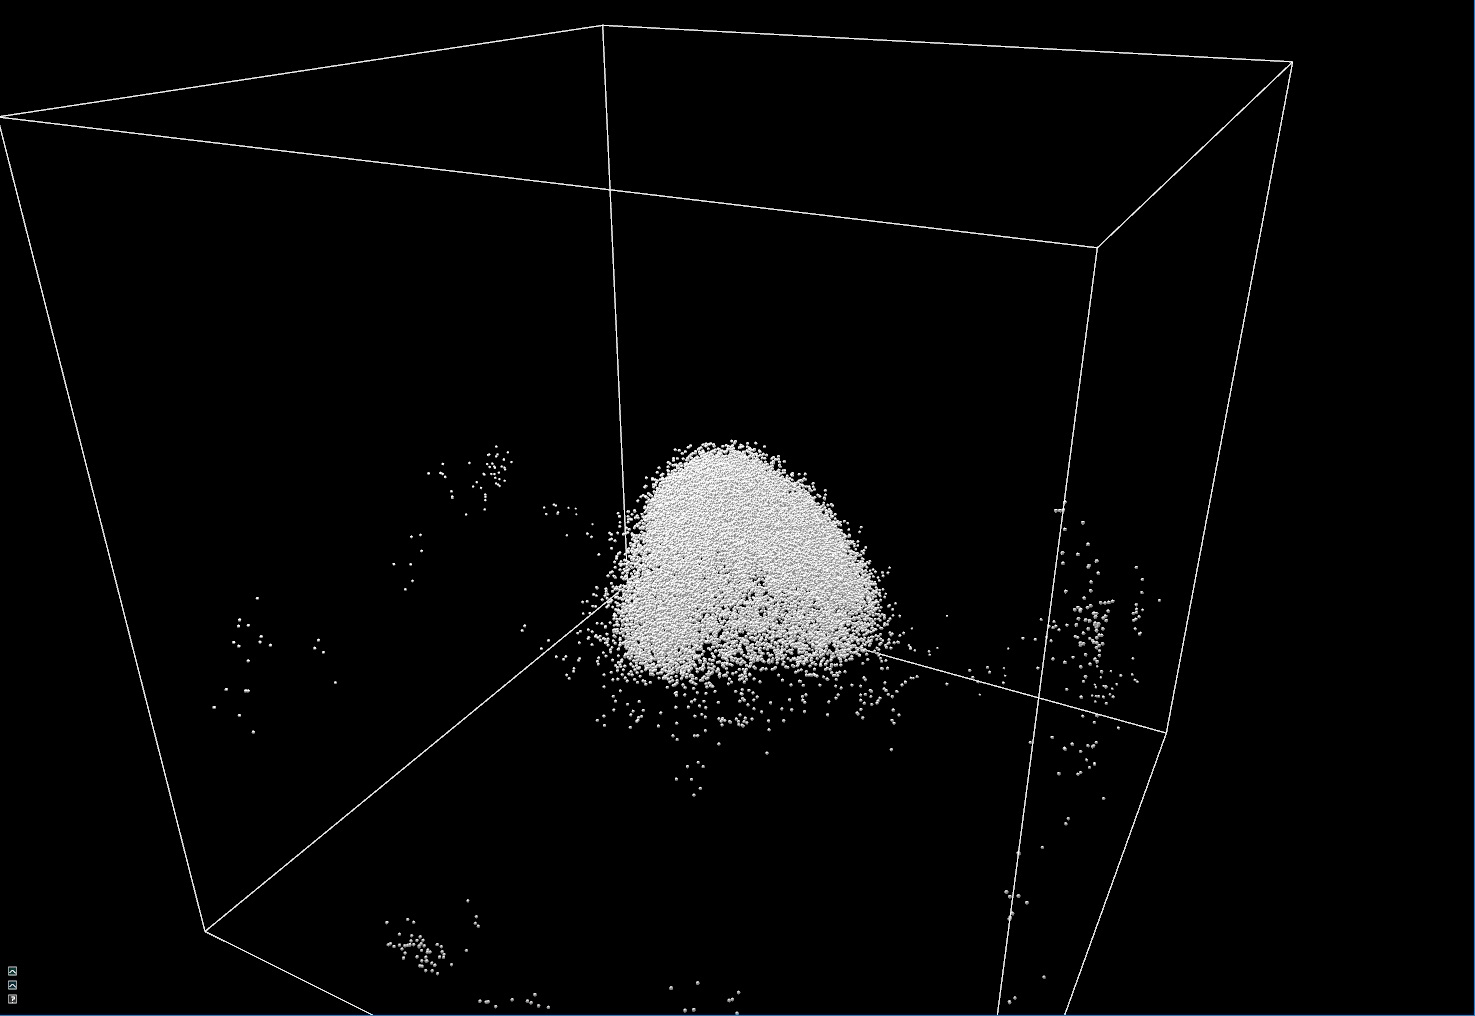
\includegraphics[width=\textwidth]{prt_jpg/11_3}
        \caption{3 részecske}
    \end{subfigure}
    \hfill
    \begin{subfigure}[!htb]{0.32\textwidth}
        \centering
        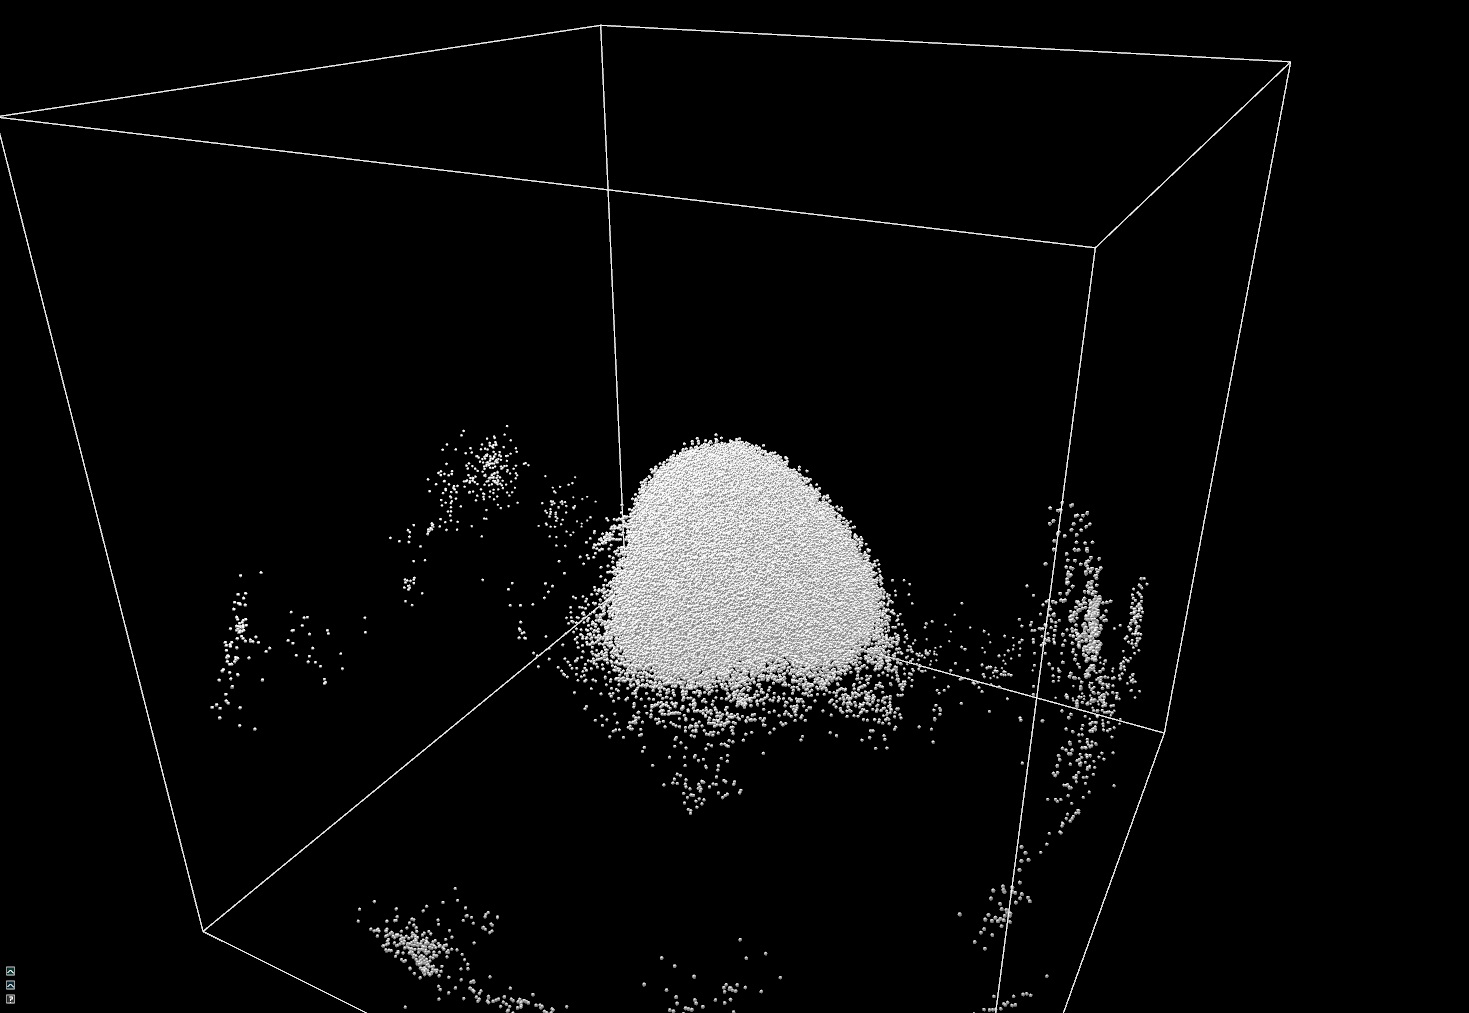
\includegraphics[width=\textwidth]{prt_jpg/11_20}
        \caption{20 részecske}
    \end{subfigure}
    \caption{A 11. frame}
    \label{fig:x frameeleven}
\end{figure}

\begin{figure}[!htb]
    \centering
    \begin{subfigure}[!htb]{0.32\textwidth}
        \centering
        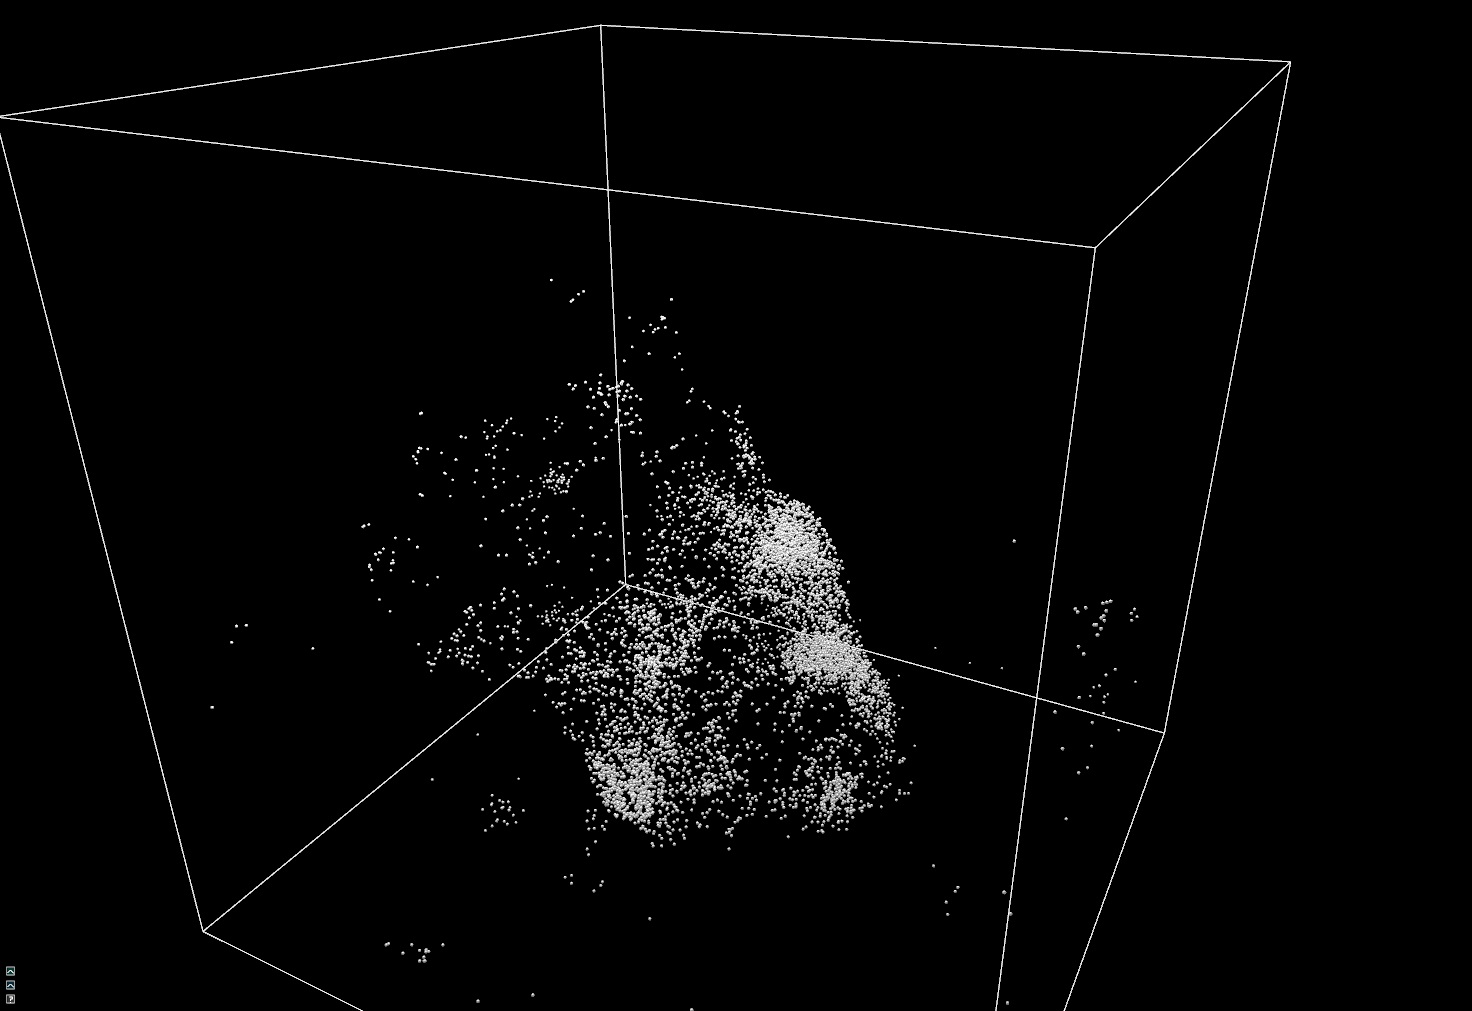
\includegraphics[width=\textwidth]{prt_jpg/14_0}
        \caption{0 részecske}
    \end{subfigure}
    \hfill
    \begin{subfigure}[!htb]{0.32\textwidth}
        \centering
        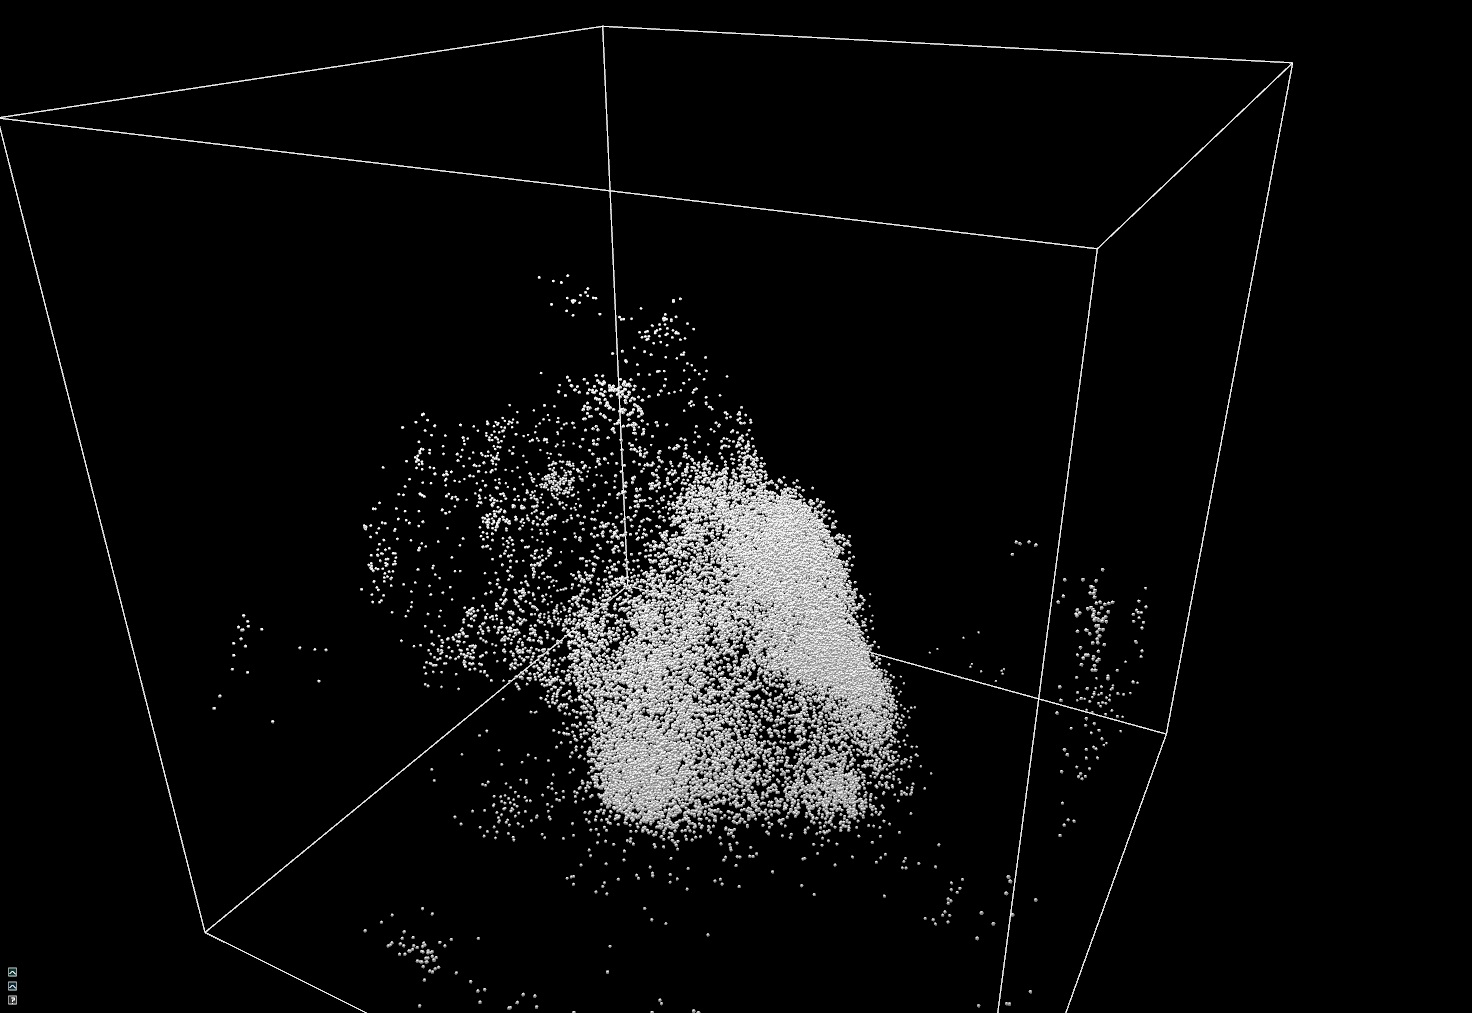
\includegraphics[width=\textwidth]{prt_jpg/14_3}
        \caption{3 részecske}
    \end{subfigure}
    \hfill
    \begin{subfigure}[!htb]{0.32\textwidth}
        \centering
        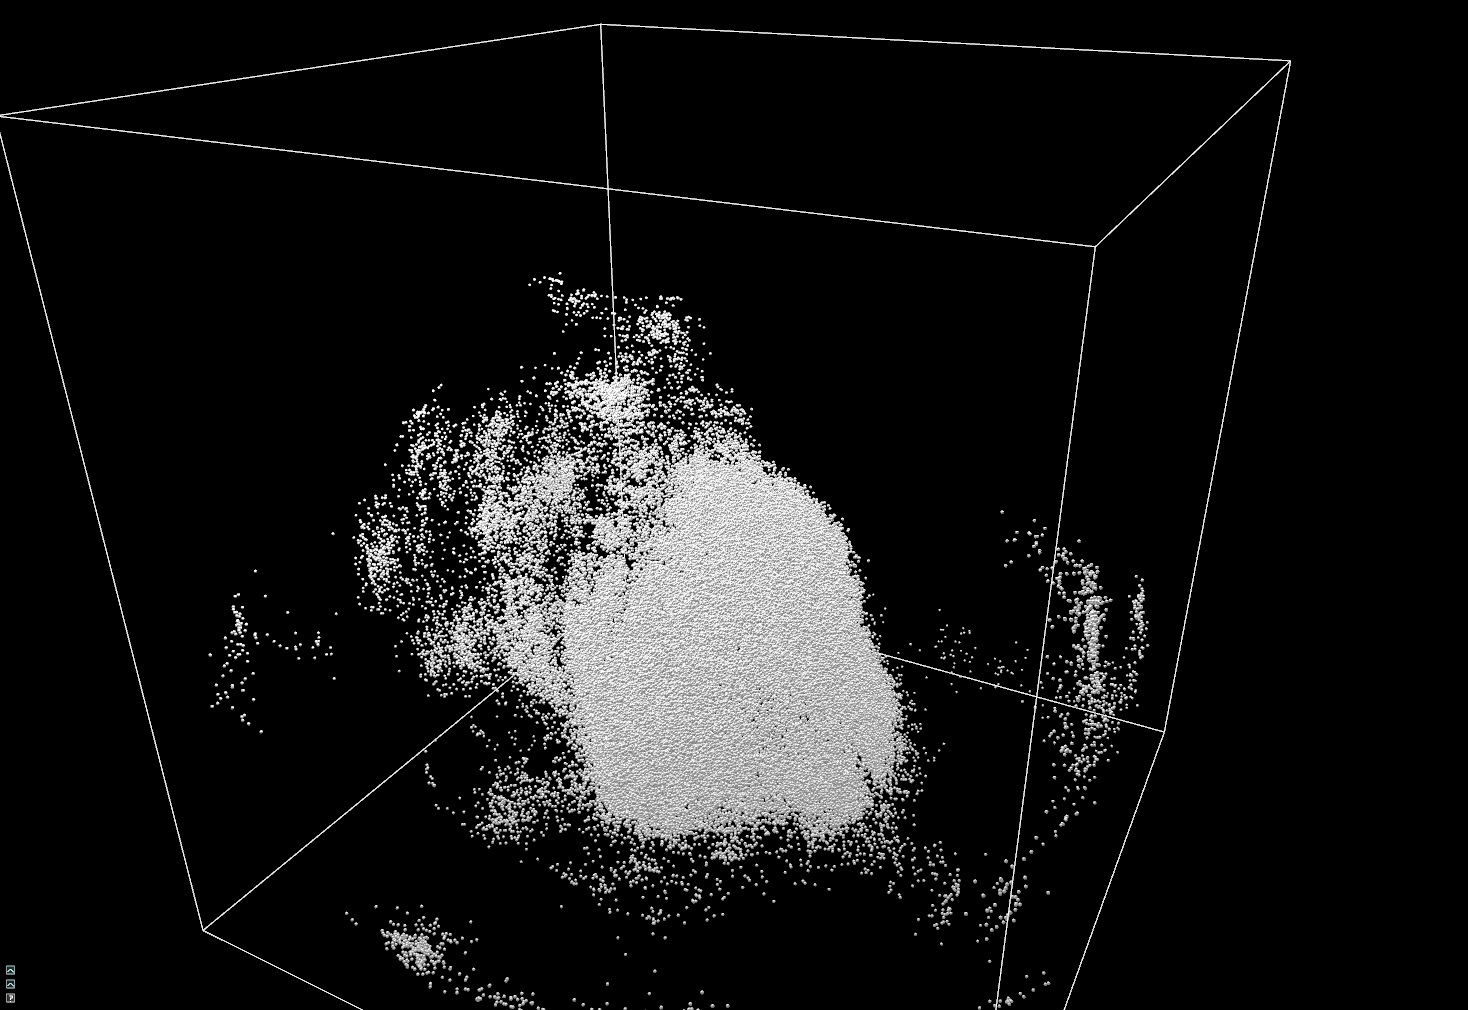
\includegraphics[width=\textwidth]{prt_jpg/14_20}
        \caption{20 részecske}
    \end{subfigure}
    \caption{A 14. frame}
    \label{fig:x frame14}
\end{figure}

\begin{figure}[!htb]
    \centering
    \begin{subfigure}[!htb]{0.32\textwidth}
        \centering
        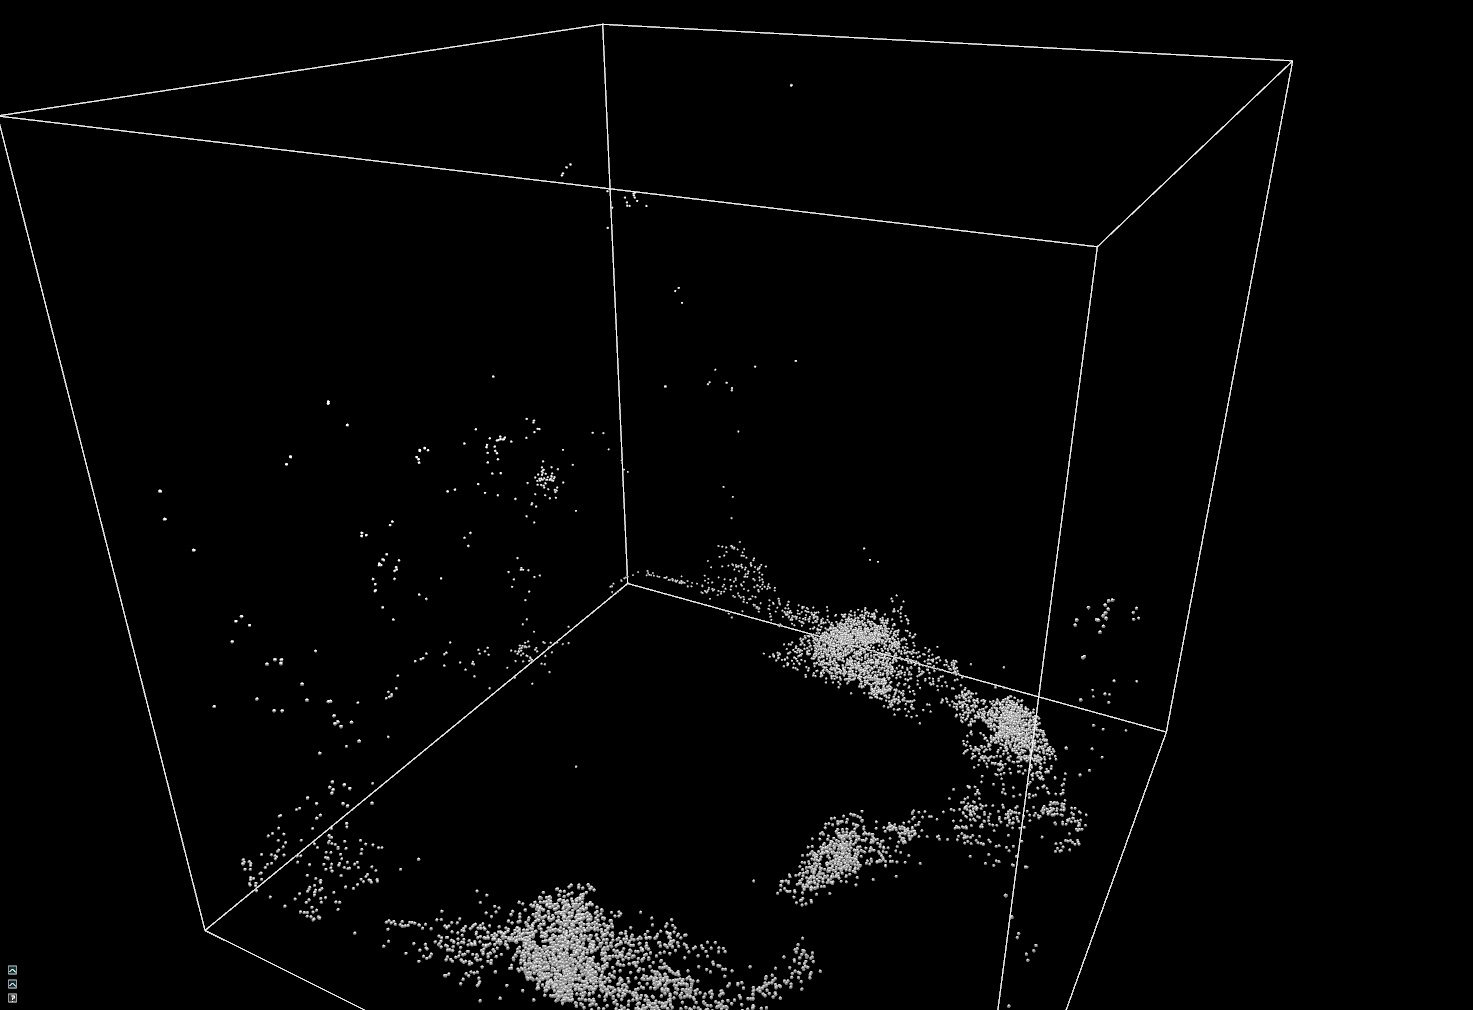
\includegraphics[width=\textwidth]{prt_jpg/30_0}
        \caption{0 részecske}
    \end{subfigure}
    \hfill
    \begin{subfigure}[!htb]{0.32\textwidth}
        \centering
        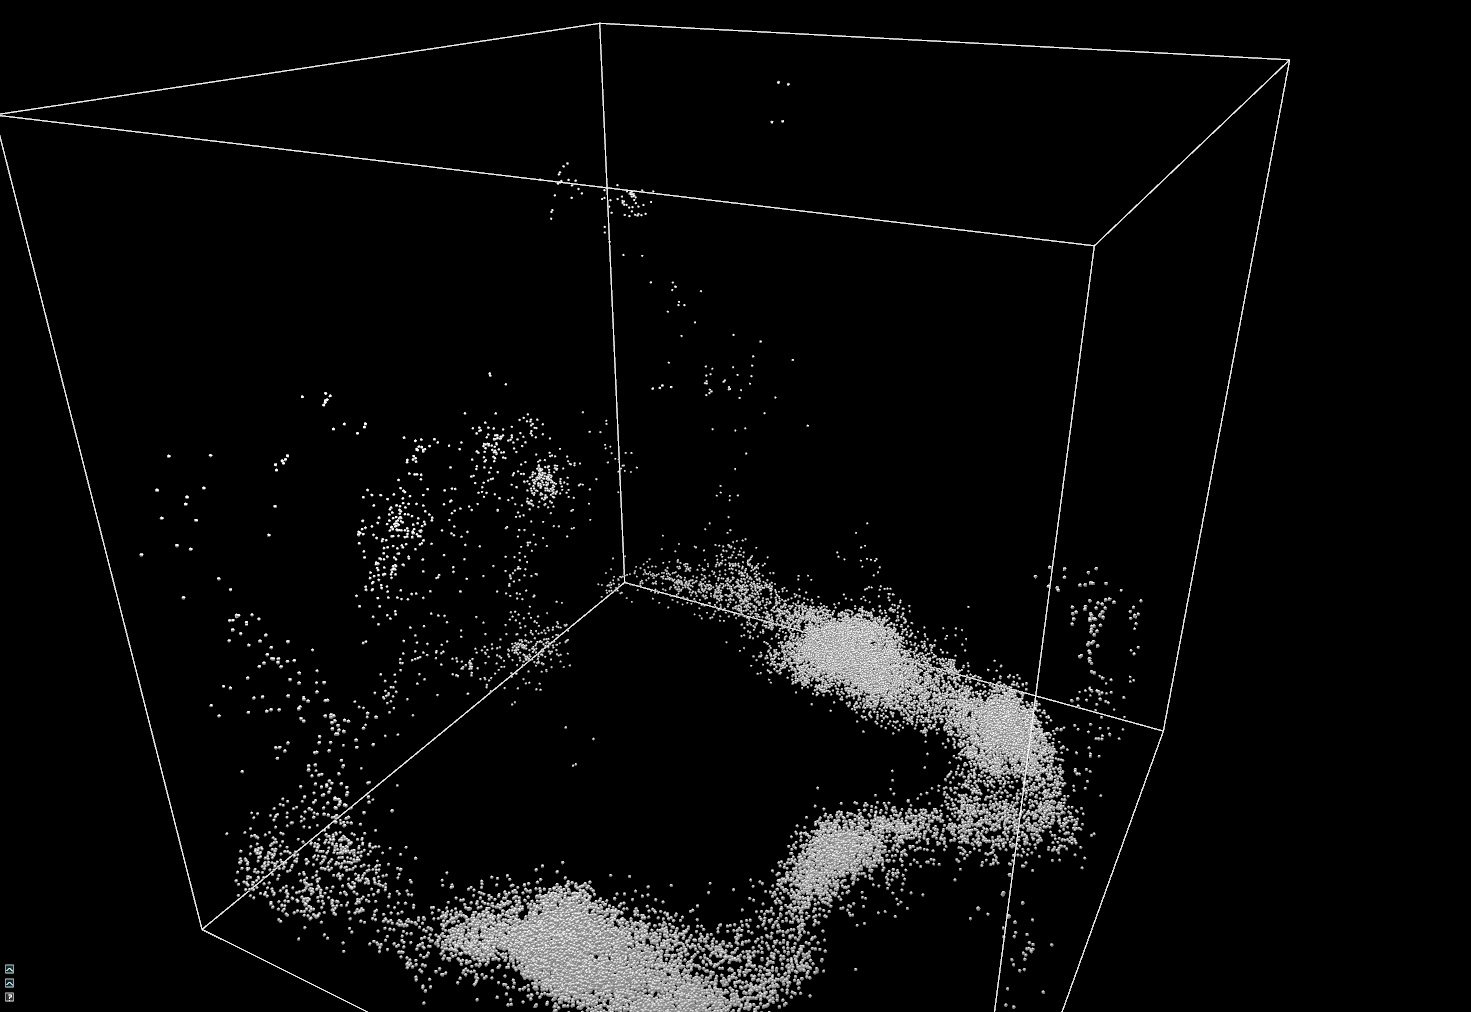
\includegraphics[width=\textwidth]{prt_jpg/30_3}
        \caption{3 részecske}
    \end{subfigure}
    \hfill
    \begin{subfigure}[!htb]{0.32\textwidth}
        \centering
        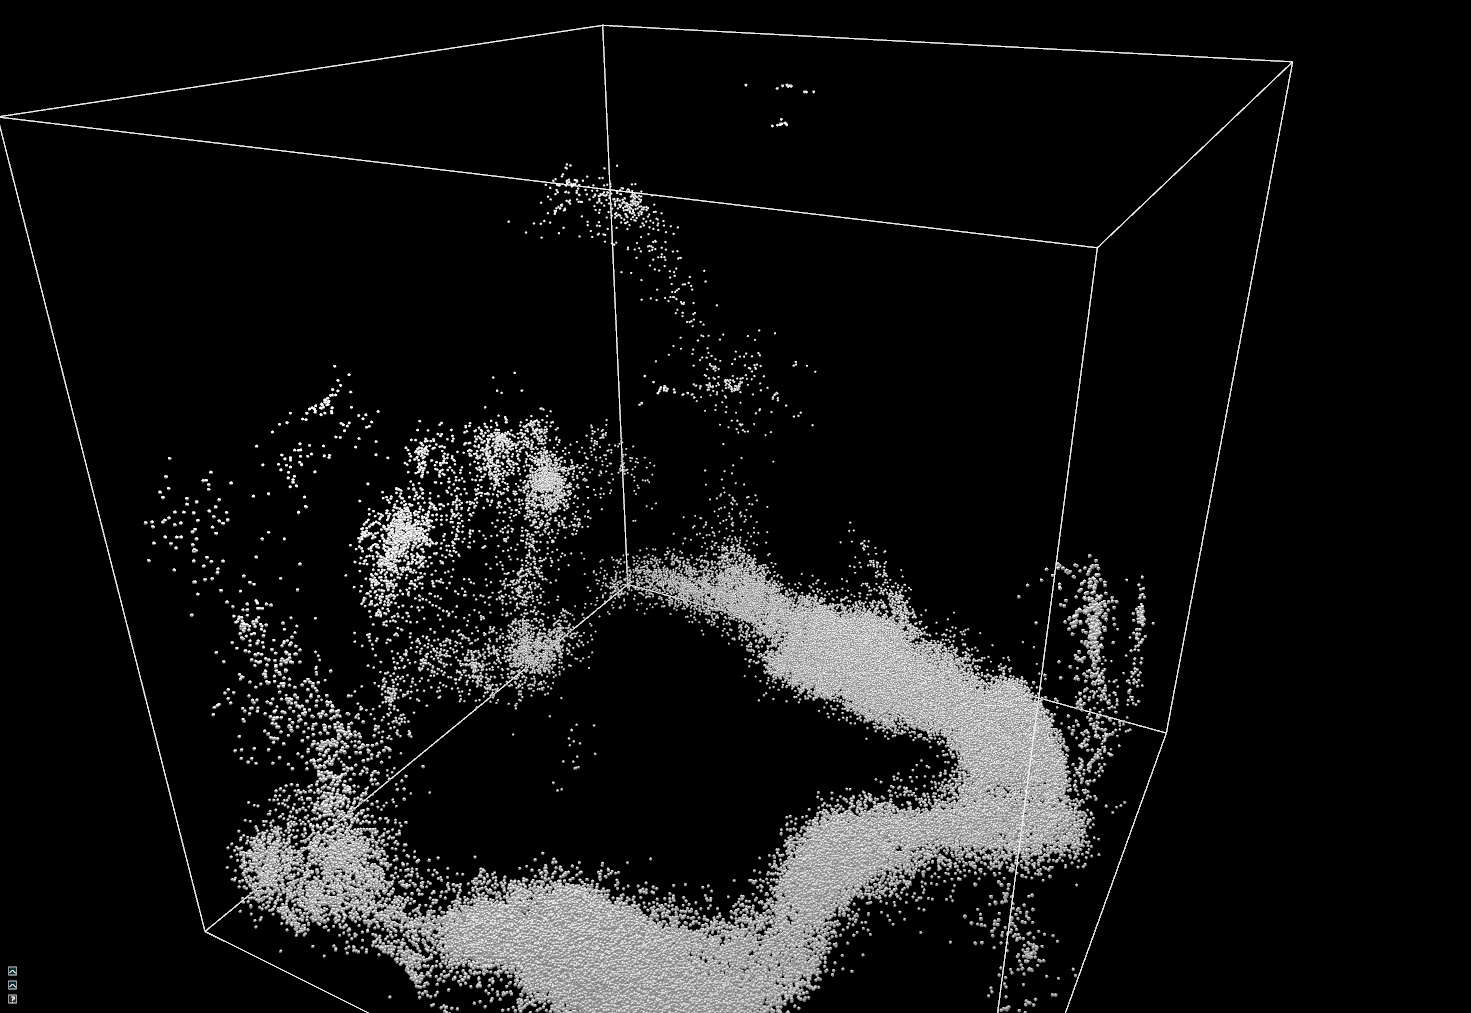
\includegraphics[width=\textwidth]{prt_jpg/30_20}
        \caption{20 részecske}
    \end{subfigure}
    \caption{A 30. frame}
    \label{fig:x frame30}
\end{figure}





